%%%%%%%%%%%%%%%%%%%%%%%%%%%%%%%%%%%%%%%%%%%%%%%%%%%%%%%%%%%%%%%%%%%%%%%%%%%%
% AGUtmpl.tex: this template file is for articles formatted with LaTeX2e,
% Modified July 2011
%
% This template includes commands and instructions
% given in the order necessary to produce a final output that will
% satisfy AGU requirements.
%
% PLEASE DO NOT USE YOUR OWN MACROS
% DO NOT USE \newcommand, \defcommand, or \renewcommand.
%
% FOR FIGURES, DO NOT USE \psfrag or \subfigure.
%
%%%%%%%%%%%%%%%%%%%%%%%%%%%%%%%%%%%%%%%%%%%%%%%%%%%%%%%%%%%%%%%%%%%%%%%%%%%%
%
% All questions should be e-mailed to latex@agu.org.
%
%%%%%%%%%%%%%%%%%%%%%%%%%%%%%%%%%%%%%%%%%%%%%%%%%%%%%%%%%%%%%%%%%%%%%%%%%%%%
%
% Step 1: Set the \documentclass
%
% There are two options for article format: two column (default)
% and draft.
%
% PLEASE USE THE DRAFT OPTION TO SUBMIT YOUR PAPERS.
% The draft option produces double spaced output.
%
% Choose the journal abbreviation for the journal you are
% submitting to:

% jgrga JOURNAL OF GEOPHYSICAL RESEARCH
% gbc   GLOBAL BIOCHEMICAL CYCLES
% grl   GEOPHYSICAL RESEARCH LETTERS
% pal   PALEOCEANOGRAPHY
% ras   RADIO SCIENCE
% rog   REVIEWS OF GEOPHYSICS
% tec   TECTONICS
% wrr   WATER RESOURCES RESEARCH
% gc    GEOCHEMISTRY, GEOPHYSICS, GEOSYSTEMS
% sw    SPACE WEATHER

% (If you are submitting to a journal other than jgrga,
% substitute the initials of the journal for "jgrga" below.)

\documentclass[draft,jgrga]{statclim}
\usepackage{amsmath} %for help with the bracketed conditional equations
\usepackage{graphicx}
\usepackage{multirow}
\usepackage{mathtools}
\usepackage{chngcntr}
\usepackage{lineno}
\linenumbers
\setkeys{Gin}{draft=false}
%%%%%%%%%%%%%%%%%%%%%%%%%%%%%%%%%%%%%%%%%%%%%%%%%%%%%%%%%%%%%%%%%%%%%%%%%
% OPTIONAL:
% To produce a two-columned version:
% \documentclass[jgrga]{AGUTeX}

% Two-columned format can be used to estimate the number of pages
% for the final published PDF.

% PLEASE USE THE DRAFT OPTION TO SUBMIT YOUR PAPERS.
%%%%%%%%%%%%%%%%%%%%%%%%%%%%%%%%%%%%%%%%%%%%%%%%%%%%%%%%%%%%%%%%%%%%%%%%%
% OPTIONAL:
% To create numbered lines:

% If you don't already have lineno.sty, you can download it from
% http://www.ctan.org/tex-archive/macros/latex/contrib/ednotes/
% (or search the internet for lineno.sty ctan), available at TeX Archive Network (CTAN).
% Take care that you always use the latest version.

% To activate the commands, uncomment \usepackage{lineno}
% and \linenumbers*[1]command, below:

% \usepackage{lineno}
% \linenumbers*[1]

%  To add line numbers to lines with equations:

%  \begin{linenomath*}
%  \begin{equation}
%  \end{equation}
%  \end{linenomath*}
%%%%%%%%%%%%%%%%%%%%%%%%%%%%%%%%%%%%%%%%%%%%%%%%%%%%%%%%%%%%%%%%%%%%%%%%%
% Figures and Tables
%
% When submitting articles through the GEMS system:
% COMMENT OUT ANY COMMANDS THAT INCLUDE GRAPHICS.
% (See FIGURES section near the end of the file.)
%
% DO NOT USE \psfrag or \subfigure commands.
%
%  Figures and tables should be placed AT THE END OF THE ARTICLE,
%  after the references.
%
%  Uncomment the following command to include .eps files
%  (comment out this line for draft format):
%  \usepackage[dvips]{graphicx}
%
%  Uncomment the following command to allow illustrations to print
%   when using Draft:
%  \setkeys{Gin}{draft=false}
%
% Substitute one of the following for [dvips] above
% if you are using a different driver program and want to
% proof your illustrations on your machine:
%
% [xdvi], [dvipdf], [dvipsone], [dviwindo], [emtex], [dviwin],
% [pctexps],  [pctexwin],  [pctexhp],  [pctex32], [truetex], [tcidvi],
% [oztex], [textures]
%
% See how to enter figures and tables at the end of the article, after
% references.
%
%% ------------------------------------------------------------------------ %%
%
%  ENTER PREAMBLE
%
%% ------------------------------------------------------------------------ %%

% Author names in capital letters:
\authorrunninghead{Muldoon et al.}

% Shorter version of title entered in capital letters:
\titlerunninghead{Byrd ice core radar dating}

% Author mailing address: please repeat this command for
% each author and alphabetize authors:

%\authoraddr{R. C. Bales,
%Department of Hydrology and Water Resources, University of
%Arizona, Harshbarger Building 11, Tucson, AZ 85721, USA.
%(roger@hwr.arizona.edu)}

%\authoraddr{J. R. McConnell, Division of Hydrologic
%Sciences, 123 Main Street, Desert Research Institute, Reno, NV
%89512, USA.}

%\authoraddr{E. Mosley-Thompson, Department of Geography,
%Ohio State University, 123 Orange Boulevard, Columbus, OH 43210,
%USA.}

%\authoraddr{R. Williams, Department of Space Sciences, University of
%Michigan, 123 Brown Avenue, Ann Arbor, MI 48109, USA.}

%\authoraddr{Francesco Visconti, Dipartimento di Idraulica,
%Trasporti ed Infrastrutture Civili, Politecnico di Torino,
%Corso Duca degli Abruzzi 24, I-10129, Torino, Italy.

\begin{document}

%% ------------------------------------------------------------------------ %%
%
%  TITLE
%
%% ------------------------------------------------------------------------ %%


\title{Bayesian estimation of englacial radar chronology in Central West Antarctica}
%
% e.g., \title{Terrestrial ring current:
% Origin, formation, and decay $\alpha\beta\Gamma\Delta$}
%

%% ------------------------------------------------------------------------ %%
%
%  AUTHORS AND AFFILIATIONS
%
%% ------------------------------------------------------------------------ %%


%Use \author{\altaffilmark{}} and \altaffiltext{}

% \altaffilmark will produce footnote;
% matching \altaffiltext will appear at bottom of page.

 \authors{Gail R. Muldoon,\altaffilmark{1,}\altaffilmark{2}$^\dagger$  Charles S. Jackson,\altaffilmark{1} Duncan A. Young,\altaffilmark{1} 
 and Donald D. Blankenship \altaffilmark{1}}

\altaffiltext{1}{University of Texas Institute for Geophysics, Jackson School of Geosciences, University of Texas at Austin, Austin, Texas, USA}
\altaffiltext{2}{Department of Geological Sciences, Jackson School of Geosciences, University of Texas at Austin, Austin, TX, USA}
%\correspondingauthor{Gail Muldoon}
$\dagger${gail.muldoon@utexas.edu}
% \authors{R. C. Bales,\altaffilmark{1}
% E. Mosley-Thompson,\altaffilmark{2} R. Williams,\altaffilmark{3}
% J. R. McConnell\altaffilmark{4}, and Francesco Visconti\altaffilmark{5}}

%\altaffiltext{1}{Department of Hydrology and Water Resources,
%University of Arizona, Tucson, Arizona, USA.}

%\altaffiltext{2}{Department of Geography, Ohio State University,
%Columbus, Ohio, USA.}

%\altaffiltext{3}{Department of Space Sciences, University of
%Michigan, Ann Arbor, Michigan, USA.}

%\altaffiltext{4}{Division of Hydrologic Sciences, Desert Research
%Institute, Reno, Nevada, USA.}

%\altaffiltext{5}{Dipartimento di Idraulica, Trasporti ed
%Infrastrutture Civili, Politecnico di Torino, Turin, Italy.}

%% ------------------------------------------------------------------------ %%
%
%  ABSTRACT
%
%% ------------------------------------------------------------------------ %%

% >> Do NOT include any \begin...\end commands within
% >> the body of the abstract.

\begin{abstract}
  Englacial radar reflectors in the central West Antarctic Ice Sheet (WAIS) contain information about past dynamics and ice properties. Due to significant data coverage in this area, these isochronous reflectors can be traced over large portions of the ice sheet, but assigning ages to the reflectors for the purpose of studying dynamics requires incorporation of chronologic data from ice cores. To date reflectors in the Marie Byrd Land region, we consider the Byrd ice core, strategically located between the catchments of Thwaites Glacier and the Siple Coast ice streams. 

Here we determine ages with uncertainty for a series of four englacial radar reflectors spanning the ice thickness using Bayesian approaches to combine radar observations, an existing Byrd ice core chronology, and a simplified ice sheet model. This method returns the joint probability distribution of depth and age for observed radar reflectors. The inferred age-depth profiles at the Byrd ice core site compare favorably with the more recent WAIS Divide ice core record. The results include inferences of accumulation rate history that show an expected decline in accumulation rate during the Last Glacial Maximum. The deepest continuous radar reflector is approximately 25.42 $\pm$ 2.49 ka, far younger than the estimated age recorded at the bottom of the ice core. 
\end{abstract}

%% ------------------------------------------------------------------------ %%
%
%  BEGIN ARTICLE
%
%% ------------------------------------------------------------------------ %%

% The body of the article must start with a \begin{article} command
%
% \end{article} must follow the references section, before the figures
%  and tables.

\begin{article}

%% ------------------------------------------------------------------------ %%
%
%  TEXT
%
%% ------------------------------------------------------------------------ %%

\section{Introduction}\label{intro}
	% Airborne ice-penetrating radar data has been used to explore past ice sheet evolution and flow as well as to indirectly probe modern ice sheet boundary conditions. In order to do so, it is useful to determine the age of radar-observed englacial layers to provide constraints on the timing of features indicative of  change within the ice. More than a dozen surveys over the last several decades have provided extensive coverage of central West Antarctica, including the Thwaites Glacier catchment and Marie Byrd Land regions. These surveys pass near the Byrd (80.0167$^\circ$S, 119.5167$^\circ$W) and WAIS Divide (79.48$^{\circ}$S, 112.11$^{\circ}$W) ice cores, making it possible to correlate ice core chronologies with observed englacial layers at depth. 

% The WAIS Divide ice core has been dated to 68 ka and the Byrd ice core has been dated to 91 ka, thus providing the potential for dating West Antarctic englacial ice through most of the Last Interglacial cycle. However, while a robust age-depth chronology is available for the recently-drilled WAIS Divide ice core, the Byrd ice core chronology -- the first deep core to be drilled in Antarctica -- lacks sufficient error analysis. We derive uncertainty for the Byrd ice core chronology using a combination of ice flow modeling and correlation of layers traced between the well-dated WAIS Divide ice core and the Byrd ice core. Additionally, the contribution of uncertainty in layer depth observed from ice-penetrating radar has not been computed for the West Antarctic. Using specifications of the radar system, we quantify radar depth uncertainty and include it when assigning ages to radar-observed layers of interest.

% Age registration of englacial layers is most practical for layers which can be tracked continually both to an ice core and throughout a large domain. We identify 9 such layers at the WAIS Divide ice core and 10 layers at the Byrd ice core which are dated and tracked for hundreds of line-km in central West Antarctica. The result is isochronous surfaces which reveal evidence of deformation in the ice sheet and could identify areas of changes in accumulation, flow, or subglacial boundary conditions. This three-dimensional view of the inside of the West Antarctic ice sheet provides a new avenue to validate ice sheet models and explore past behavior and dynamics of the ice sheet. 

% \begin{figure}[!h]
% %\begin{center}
% \centering
% \includegraphics[scale=0.3]{figures/Fig1_WAISall_bed2}
% %\captionsetup{width=.9\textwidth}
% \caption[]{Map of central West Antarctic with available airborne geophysical radar surveys (black lines) and (\textbf{will be updated to have:} WAIS Divide and Byrd ice core locations (blue triangles) overlain. Gray shading is surface elevation according to Fretwell et al. 2013. }
% %\end{center}
% \label{fig:radarmap}
% \end{figure}

% Start version from 2 Aug 2017%
%The Byrd ice core (80.0167$^\circ$S, 119.5167$^\circ$W) was the first to be drilled to bedrock in Antarctica \citep{gow1968}. The proximity of the core to fast-changing ice of both the Siple and Amundsen Sea coasts in West Antarctica makes it a potentially important source of information in studies of the response of the West Antarctic Ice Sheet (WAIS) to changing climatic conditions. More than three extensive radar surveys pass near the core site, including the recent GIMBLE survey filling a data coverage gap in Marie Byrd Land \citep{duncan}, make it particularly useful for dating paleo ice dynamics observed in the central WAIS. Dated englacial radar data enables information from the entire ice volume--rather than only surface observations--to constrain ice dynamics in the central WAIS, including the Thwaites Glacier catchment and Marie Byrd Land.

%While the Byrd ice core has been dated to more than 90ka \citep{}, nearly back to the Last Interglacial, the chronology lacks estimates of uncertainty in age and depth. Here we use a Bayesian technique to compute a probabilistic chronology for the Byrd ice core which is constrained by existing ice core chronology results. This method inverts for probability distributions of ice sheet parameter values consistent with the recorded ice core chronology. 

%We use the modeled chronology to assign ages to englacial reflectors traced through the central WAIS. These reflectors encode information about ice sheet boundary conditions and paleo ice dynamics \citep[e.g.][]{}. They are the result of dielectric contrasts in the ice due to variations in composition, crystal fabric, temperature, and other ice properties. Each continuous reflector is assumed to be the result of a distinct surface deposition episode with a distinguishable dielectric signature and is therefore assumed to be isochronous \citep{fujita2000}. 

%The isochronous nature of englacial reflectors implies that assigning an age to each reflector at the Byrd ice core site effectively dates the reflector anywhere it can be continuously traced in the region. This allows for extensive age registration throughout the ice column and radar survey domain and also for validation of our results at the Byrd ice core with the recently-drilled WAIS Divide ice core chronology, as has been done in East Antarctica \citep{cavitte2016}. The WAIS Divide ice core (79.48$^{\circ}$S, 112.11$^{\circ}$W) provides an ice chronology with uncertainty quantification as far as back as 67ka \citep[][C. Buizert, personal communication]{buizert2015} and is therefore an independent validation of our improved Byrd ice core chronology. 

%Having two ice cores from which to date englacial reflectors enables more extensive dating, particularly in areas of complicated basal topography where the radar isochrones experience increased discontinuity and cannot be tracked for long distances. This is the case near the Marie Byrd Land icecap, for example, where reflectors present at the Byrd ice core site have been traced around areas of disruption due to high-relief bed terrain. In general, deeper reflectors are more difficult to track extensively in the WAIS due to lower reflection amplitudes and increased disruption. However, we interpolate three-dimensional isochronous surfaces for the extent of each of four observed reflectors which sample the ice depth. The modeled chronology is used to assign ages to these surfaces.

%End version from 2 Aug 2017%

Isochronous, englacial radar reflectors observed by ice-penetrating radar record the depth and extent of isosurfaces with shared physical properties \citep{siegert1998,dowdeswell2004}. These reflectors can map the age structure of an ice sheet, with the thickness of layers bounded by reflectors revealing information about ice flow dynamics and variable ice properties. Such observations have been used in Greenland and Antarctica to infer the ice flow history of the ice sheets in response to changing climate regimes in the past \citep{macgregor2015}. To provide such historical climatic context, reflectors are assigned ages by correlation to a known chronology, such as at an ice core site \citep{cavitte2016}. Dating englacial reflectors enables information from the entire ice volume, not only surface observations, to constrain ice sheet dynamics. However, combining information from ice cores and radar observations is intrinsically complicated by the fact that ice core chronologies assign discrete ages to samples of ice, while radar reflectors track packets of ice with finite thickness that span a range of ages, particularly at depth where age is more sensitive to depth due to shear thinning of the ice. 

To understand how well radar reflectors can be dated, we use Bayesian methods %\citep{metropolis1953,hastings1970,gelfand1992} 
to synthesize information from ice cores, radar sampling, ice flow modeling, and our knowledge of the leading sources of uncertainty within the radar and ice core data sources. We apply our approach to the central West Antarctic Ice Sheet (WAIS), an area containing the potential for unforced retreat where ice dynamics are of particular interest for projections of future sea level rise. In addition to being of scientific importance, the central WAIS is an area with concentrated radar surveys and two deep ice cores, the Byrd ice core \citep{gow1968} and the WAIS Divide ice core \citep{buizert2015}. In particular, the proximity of the Byrd ice core (80.0167$^\circ$S, 119.5167$^\circ$W) to fast-changing ice of both the Siple and Amundsen Sea coasts in West Antarctica makes it a potentially important source of information about the response of the WAIS to climate change.
%In particular, the proximity of the Byrd ice core \cite[(80.0167$^\circ$S, 119.5167$^\circ$W),][]{gow1968} to fast-changing ice of both the Siple and Amundsen Sea coasts in West Antarctica makes it a potentially important source of information in studies of the response of the West Antarctic Ice Sheet (WAIS) to changing climatic conditions.

The Byrd ice core is co-located with several extensive radar surveys (Figure~\ref{fig:radarmap}) and contains an ice record that extend back to more than 90 ka \citep{blunier2001}, nearly back to the Last Interglacial. Rather than use existing chronologies for the age-depth relationship at the Byrd ice core, which do not sufficiently characterize its uncertainty, we generate our own chronologies using Bayesian strategies to synthesize an ice flow model with age-depth data obtained from volcanics sampled from the Byrd ice core \citep{gow1968,gow1970,hammer1997}. This method allows us to simulate the co-dependence in dating errors within and between different radar reflectors.

The four reflectors in this study were chosen as a representative sample of the ice column and for their signal-to-noise ratio and continuity. It is possible to use this method to date additional englacial reflectors observed using radar in this area, but the usefulness of such ages extend only as far as the isochronous reflectors can be horizontally traced. While this method is less helpful for dating discontinuous reflectors, it could inform relative ages for sections of discontinuous reflectors adjacent to dated reflectors in the ice column  \citep[e.g.][]{macgregor2015}.

%However, there are currently no formal estimates of uncertainty in its chronology. Quantifying such uncertainty is challenging because it arises from a number of sources, including measured depth and age of the ice and unknown local ice flow parameters. This problem is nontrivial because age-depth solutions are nonunique and depend on solutions elsewhere in the ice column. Despite this, it is important to include uncertainty in the Byrd ice core chronology when using it to characterize the englacial age structure of the greater WAIS to limit the propagation of unrealistic certainty in age, particularly at depth where shear thinning is dominant and uncertainties are expected to be greatest. 

We consider two quantities of interest in this problem: radar-inferred depths from observed two-way travel time (TWTT) and dated volcanics from the Byrd ice core. The primary sources of uncertainty in radar depths include the speed of electromagnetic radiation in ice, the density and thickness of the firn layer, and radar range precision. The error on range precision is determined independently for each reflector and the ice surface, while errors in velocity and firn are systematic (common) across all reflectors of interest in the ice column which are deeper than the firn layer. To estimate the ages of reflectors, we make use of dates determined for volcanic markers in the ice column \citep{hammer1997}. %However, we must estimate age errors in the absence of published uncertainty on the volcanic record. 
In the absence of published uncertainty in the volcanic record, we use a Bayesian strategy to include an uncertain age uncertainty.
An ice flow model is used to smoothly transfer information from the volcanics to the estimated depth of our reflectors of interest. To do so, it is necessary to infer flow physics parameters and accumulation rate history. Estimated ice flow and accumulation rate parameters are dependent on one another and on depth and are applied to the full ice column. A Bayesian framework allows us to describe all  components of the problem within a single calculation, but requires stochastic sampling to estimate the marginal probability of reflector depth (and therefore age) as a function of observed TWTT and volcanics.



%We use a novel approach to probabilistically date englacial radar reflectors observed near the Byrd ice core given information about the radar-observed two-way travel time (TWTT), previously-computed age-depth observations of the ice core, constraints on englacial stratigraphy, and other factors. A simple flow model is used to show how age of the reflectors varies with depth, taking into account our knowledge of ice flow physics and surface accumulation rate. While some information about these parameters is known, large uncertainties remain. To account for these uncertainties and nonunique solutions of the age-depth chronology, we use a probabilistic method to estimate uncertainty in the parameter values to find combinations of parameter values which lead to age-depth solutions consistent with observations.



%The estimated Byrd ice core chronology and published WAIS Divide ice core record are used to assign dates to englacial radar reflectors observed at the ice core sites, which are assumed isochronous \citep{cite}. These isochronous reflectors have been traced extensively throughout Central West Antarctica. As such, we leverage the ice core chronologies to date observable ice stratigraphy hundreds of kilometers from existing ice core records.


Section~\ref{byrdchronology} discusses the formulation of the Bayesian problem and methods for finding solutions of the age and depth of observed englacial radar reflectors. Section~\ref{agedepthresults} shows results for the probability distributions of reflector age and depth as well as a comparison to the WAIS Divide ice core chronology as an independent check on our results. %Section~\ref{layersurfaces} explores the application of ages at the ice cores to extensive isochronous surfaces throughout West Antarctica, which can be used to analyze paleo flow and boundary conditions in the region. 
We also calculate an error budget to determine the dominant contributions to age-depth uncertainty, discussed in Section~\ref{discussion}.


\section{Posterior distribution of englacial reflector age-depth}\label{byrdchronology}
	
% An age profile with associated errors is available at the WAIS Divide ice core site (Buizert, personal communication 2016), however the  site lacks a robust measure of uncertainty. To derive Byrd ice core, we use volcanic events  detected in the Byrd ice core using the electrical conductivity method \citep{hammer1997}. We assume a 3\% uncertainty on the volcanic ages as a rule of thumb (personal communication, T.J. Fudge). We then invert for age given layer depth using a Bayesian MCMC approach and check our result by correlation to the nearby WAIS Divide ice core chronology.

% Our approach uses a Metropolis algorithm to fit an ice flow model to the observed volcanic profile from the Byrd ice core. An ensemble of well-fitting ice flow models is generated from this process which samples uncertainty in age given uncertainty in depth. We then sample from this ensemble to construct a distribution of likely ages for layers of interest. This method allows us to build a model using data from the last 50,000 years which can be used to estimate uncertainties in the chronology at earlier times.

In order to assign ages to observed radar reflectors, we are interested in combining information from radar, ice flow physics, and ice cores to derive an age-depth profile of ice at the Byrd ice core site. To derive this updated chronology with uncertainty, we compute the age of englacial reflectors given information about radar-observed TWTT, local ice flow, and a volcanic chronology of the ice core.

We represent the solution as an ensemble because the presence of non-unique solutions necessitates a probabilistic approach. To estimate the age-depth profile at the Byrd ice core, we use Bayesian calibration to invert for the age and depth of observed englacial radar reflectors. This problem is nontrivial because the age of each reflector depends on solutions elsewhere in the ice column, so they are correlated to each other with depth. 

This method preserves the chronologic superposition of the ice column and correlation of errors with depth, estimates the probability of ice flow parameter values, and develops a probabilistic estimate of the age-depth profile. A probabilistic approach is useful because while some parameters are well known, others are highly uncertain, such as the accumulation function at this site over time. By iteratively inverting for non-unique solutions, we find a distribution of sets of parameter values which are consistent with observations. Specifically, we derive an ensemble of age-depth profiles for the Byrd ice core constrained by agreement with a chronology of volcanic events from the past 50,000 years detected in the Byrd ice core record using the electrical conductivity method \citep{hammer1997} and with TWTT to bright, continuous reflectors observed in ice-penetrating radar \citep{holt2006,young2012,morse2002} and traced using Landmark seismic interpretation software produced by Halliburton.


%\textbf{MOVE We assume a base level of 1\% uncertainty on the volcanic ages and include a precision parameter, \textit{S}, to quantify additional uncertainty. We invert for age given depth using a Bayesian Markov Chain Monte Carlo approach and check our result by correlation to the nearby WAIS Divide ice core chronology.}

The Bayesian formulation of this problem is:
\begin{equation}\label{eqn:bigproblem}
\begin{split} %allow line break
%\begin{flalign}
%\begin{aligned}
p(A_r)  \sim  p(D_r,\vec{f},d_{firn},v_{ice},S | TWTT_r,A_{IC},D_{IC})  \propto & \\
 p(D_r,f,S) \cdot p(d_{firn})\cdot p(v_{ice}) \cdot p(A_{IC},D_{IC} | \vec{f},S&)    \cdot p(TWTT_r | D_r,d_{firn},v_{ice})
%\end{flalign}
%\end{aligned}
\end{split}
\end{equation}

Computing the posterior probability distribution of reflector ages (far left in Equation~\ref{eqn:bigproblem} requires estimating the depths of the englacial reflectors of interest ($D_r$), ice flow model parameters ($\vec{f}$), firn depth correction ($d_{firn}$), radar velocity in ice ($v_{ice}$), and precision of the Byrd ice core chronology ($S$). We estimate these values given information about observed radar reflector two-way travel time ($TWTT_r$) and the age-depth profile from the Byrd ice core volcanic record ($A_{IC}$, $D_{IC}$). 


Priors, the first three terms on the right-hand side of Equation~\ref{eqn:bigproblem}, are used to put physical bounds on estimates of quantities of interest as described in the following sections. Priors on ${D_r}$ also preserve stratigraphic dependence of radar reflectors, requiring deeper reflectors be older than shallower reflectors. Likelihood functions, the remaining two factors on the right-hand side of Equation~\ref{eqn:bigproblem}, describe the probability that modeled results agree with observations. In the first, agreement between flow model results ($\vec{f}$) and the volcanic record ($A_{IC}$,$D_{IC}$) given precision ($S$) and in the second, agreement between observed two-way travel time ($TWTT_r$) and modeled reflector depths ($D_r$) given information abou tthe local firn correction ($d_{firn}$) and radar velocity in ice ($v_{ice}$). These elements of Equation~\ref{eqn:bigproblem} are discussed more thoroughly in subsequent sections.

Accepted solutions are expected to satisfy all of these conditions simultaneously, so we take the product of their probabilities in Equation~\ref{eqn:bigproblem}. The Metropolis algorithm is used to identify combinations of parameters and boundary conditions consistent with observations and sources of uncertainty. To do so, sets of parameter values for $D_r$, $\vec{f}$, $S$, $d_{firn}$, and $v_{ice}$ are proposed using a markov chain method as in Equation~\ref{eqn:proposal}. %This method allows us to build a model using data from the last 50,000 years which can be used to estimate uncertainties in the chronology at earlier times.
Likelihood functions for age and TWTT are evaluated to accept or reject these proposed parameter sets based on how well they agree with data. Solutions are those parameter sets which are simultaneously consistent with physical limits defined by the priors and with uncertain observations. 

The resulting posterior probability distribution, $p(D_r, \vec{f},S | TWTT_r, A_{IC}, D_{IC})$, can then be used to deterministically compute the corresponding probability distribution of the age of observed radar reflectors, $p(A_r)$, using the flow model described below.


\subsubsection{Ice flow model at the Byrd ice core}
%This is consistent with experiment opinion that ice core age uncertainty is generally 2-3$\%$ of ice age (T.J. Fudge, private communication). Therefore, we construct an age-depth distribution for the Byrd ice core using statistical methods and an assumed 3$\%$ age uncertainty. The derived age-depth profile is then compared to the WAIS Divide profile using englacial layers that have been tracked between the two ice core sites. 

Due to the inherent stratigraphic dependence of age in the ice column, we use a flow model to simulate the age-depth relationship. We use a simple, one-dimensional model of ice flow (Equation \ref{schwander}) which derives ice age from accumulation and strain rate, assuming constant horizontal strain rate in the upper part of the ice sheet and a shear layer of thickness $h$ at the bottom of the ice sheet, for which we invert \citep{schwander2001}. In the shear layer, the strain rate is assumed to decrease linearly and the bottom of the ice is assumed sliding with velocity $q$ $\cdot$ $v_0$, where $v_0$ is the horizontal velocity at the surface.

\begin{equation}\label{schwander}
A(z) = \int_{z}^{H} \frac{dz}{\epsilon_z \dot{a}(z)}
\end{equation}
where
\begin{center}
$    \epsilon_z=
    \begin{cases}
                 1-k(H-z), & h \leq z \leq H \\
                  kz(q+\frac{1-q}{2h}z), & 0 < z < h
    \end{cases}, 
$
$
k = \frac{2}{2H - h(1-q)}
$
\end{center}
$H$ is ice thickness in ice equivalent, $z$ is height above the bed, $h$ is the depth to the shear layer, $\dot{a}$ is the layer thickness, and $q$ is a constant for which we invert. 

The ice flow model accounts for two primary factors in the age-depth profile: burial as a function of accumulation rate, $\dot{a}$, and thinning as a function of strain, $\epsilon_z$. In the simplest realization, ice deposited at a given time at the ice sheet surface will be found at a depth in the ice sheet corresponding to the amount of subsequent accumulation. However, due to strain thinning at depth, the ice will be less deep than would be expected if accumulation alone is considered. 

In Section~\ref{metrop}, we invert for the flow parameters $h$, $q$, and $\dot{a}$. Constant values for $h$ and $q$ are sampled from uniform priors defined in a conservative range. Accumulation is estimated for 11 units of depth spaced every 200 m starting from the ice surface and are sampled from the same uniform prior.

\begin{center}
%\begin{equation}
$p(\vec{f}) = 
	\begin{cases}
		p(h) \sim U(0, 0.5) \\
		p(q) \sim U (0, 1) \\
		p(\dot{a}_{z < 200 m ... z > 2000 m}) \sim U(0.5~m/a,0.15~m/a)\\
	\end{cases}
$	
%\end{equation}	
\end{center}

The prior distributions of flow parameters, together denoted as $p(\vec{f})$, assume the shear layer is in the bottom half of the ice sheet depth and that the bed of the ice sheet is moving slower than the surface. Accumulation as a function of depth, $\dot{a}$, is sampled from 11 distinct depth bins spanning the ice thickness. This allows for variability of accumulation over time, as expected. To limit unrealistic variability in accumulation between depth bins, Tikhonov regularization is used on the age likelihood function to punish estimates of the accumulation function which are highly-variable relative to a solution computed with no regularization and smoothed over a moving 600-m depth window.




\subsection{Radar depth and error model}
 Radar pulses transmitted into the ice sheet reflect off surfaces of dielectric contrast in the ice that are the result of variations in ice fabric, composition, temperature, and rheology of ice \citep{fujita2000}. The reflected signal is received by the radar system and recorded as two-way travel time (TWTT) from transmission to receipt.  The reflector data in this analysis (Figure~\ref{fig:layergram}) were collected by the University of Texas Institute for Geophysics, including GIMBLE \citep{gimble2017}, AGASEA \citep{holt2006}, CASERTZ \citep{morse2002}, and SOAR/WMB \citep{luyendyk2003} (Figure~\ref{fig:radarmap}). Data used to trace reflectors between Byrd ice core and WAIS Divide ice core were collected from a DC-3 or Twin Otter airborne platform and used the HiCARS coherent radar system with 60 MHz center frequency and 15 MHz bandwidth \citep{peters2005}.% or the TUD-derived incoherent radar sounder \citep{blankenship2001} with 4 MHz bandwidth.

\begin{figure}[h]
\centering
\makebox[\textwidth][c]{
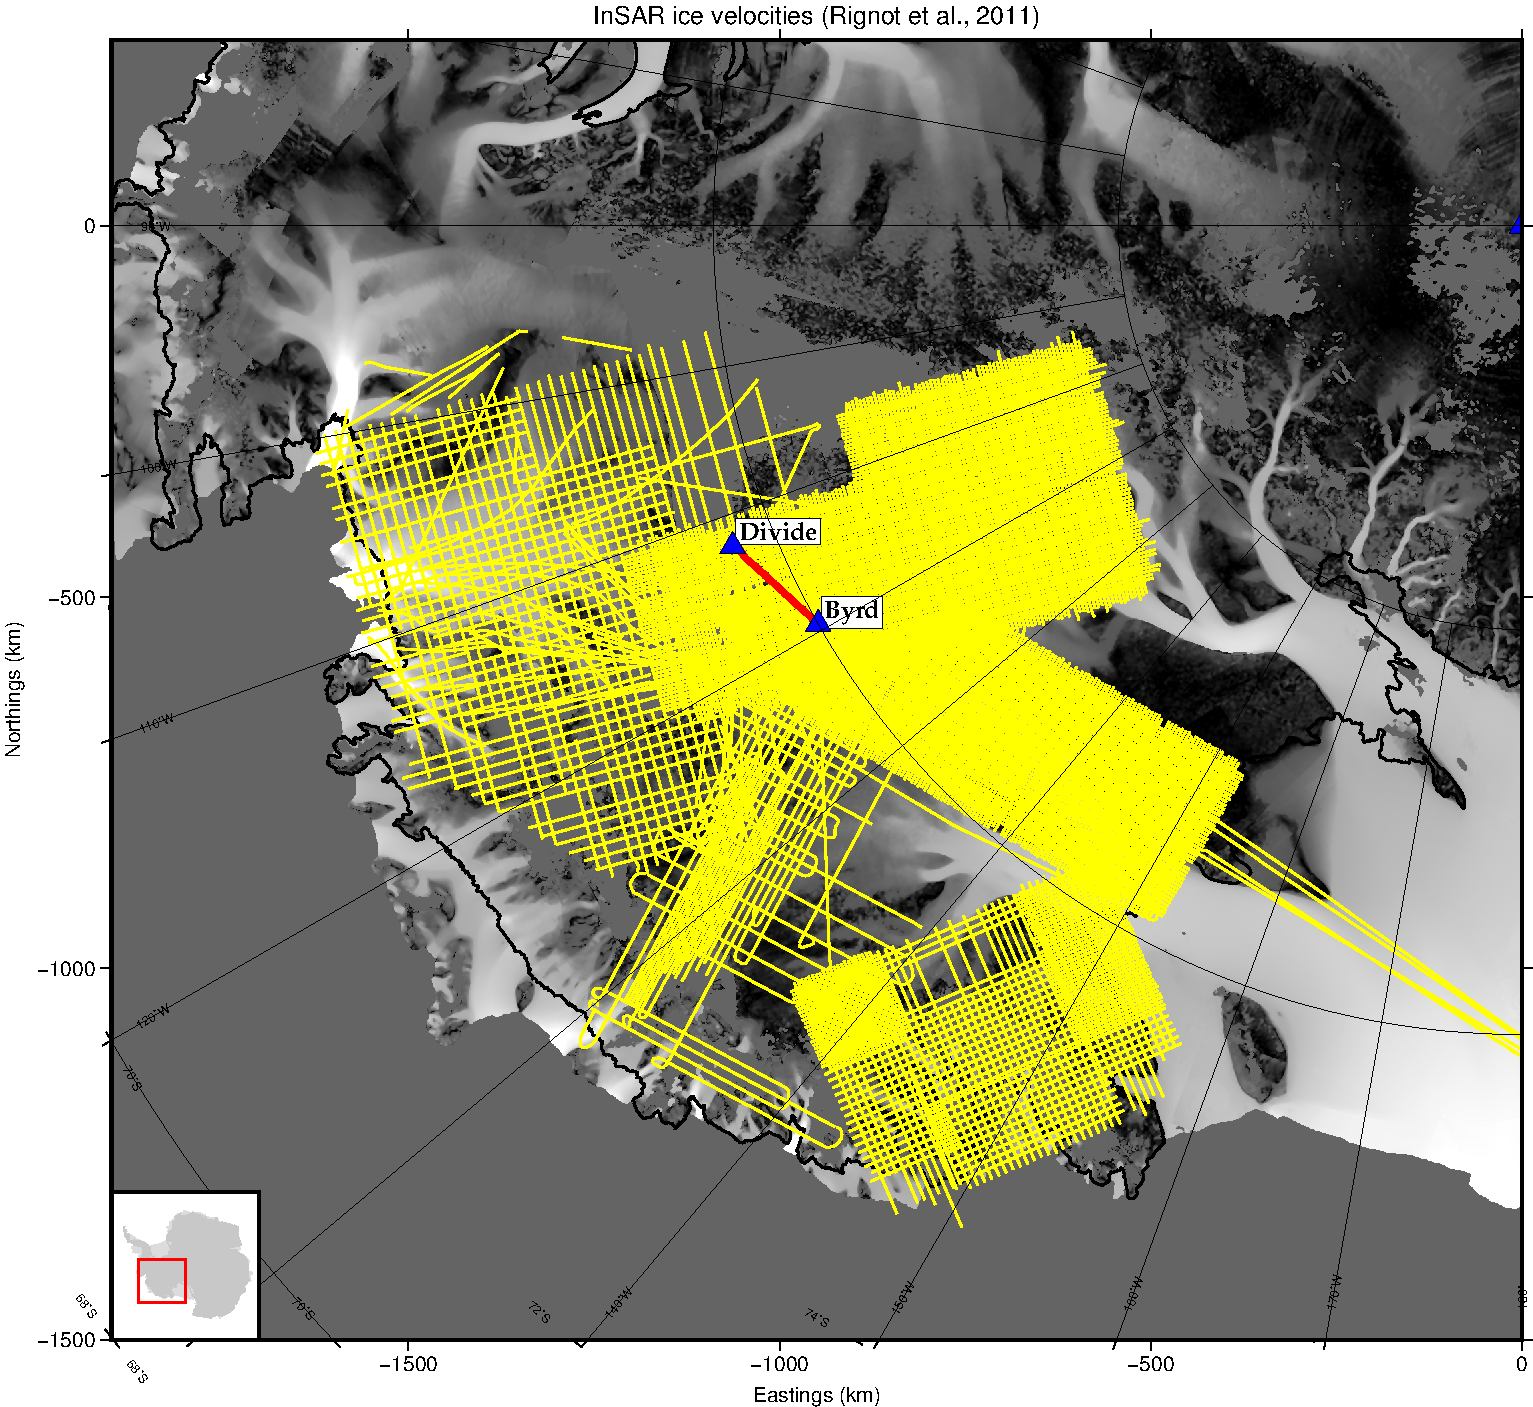
\includegraphics[scale=0.5]{/Users/gail/Documents/Research/Projects/Layers/analysis/figures/WAIS_vel_gray_final}}
%\captionsetup{width=.9\textwidth}
\caption{Map of central West Antarctic with available airborne geophysical radar surveys (yellow lines) and  WAIS Divide and Byrd ice core locations (blue triangles) overlain. Gray shading is surface velocity \citep{rignot2011}. The red line denotes the flight line along which the reflectors in this study were observed. }
\label{fig:radarmap}
\end{figure}



In this study, we consider TWTT of four reflectors spanning the ice thickness in the region of central West Antarctica (Figure~\ref{fig:layergram}). These reflectors have been tracked using Halliburton's Landmark seismic interpretation software and can be tied to both the Byrd and WAIS Divide ice cores for dating using observations from the HiCARS system (Figure~\ref{fig:radarmap}). %Determining the depth of the reflectors, $D_r$, may be affected by several sources of uncertainty, including uncertainty in the firn depth, the velocity of the radar pulse in ice, and the pulse-limited precision of radar observations.

\begin{figure}[h]
\centering
\makebox[\textwidth][c]{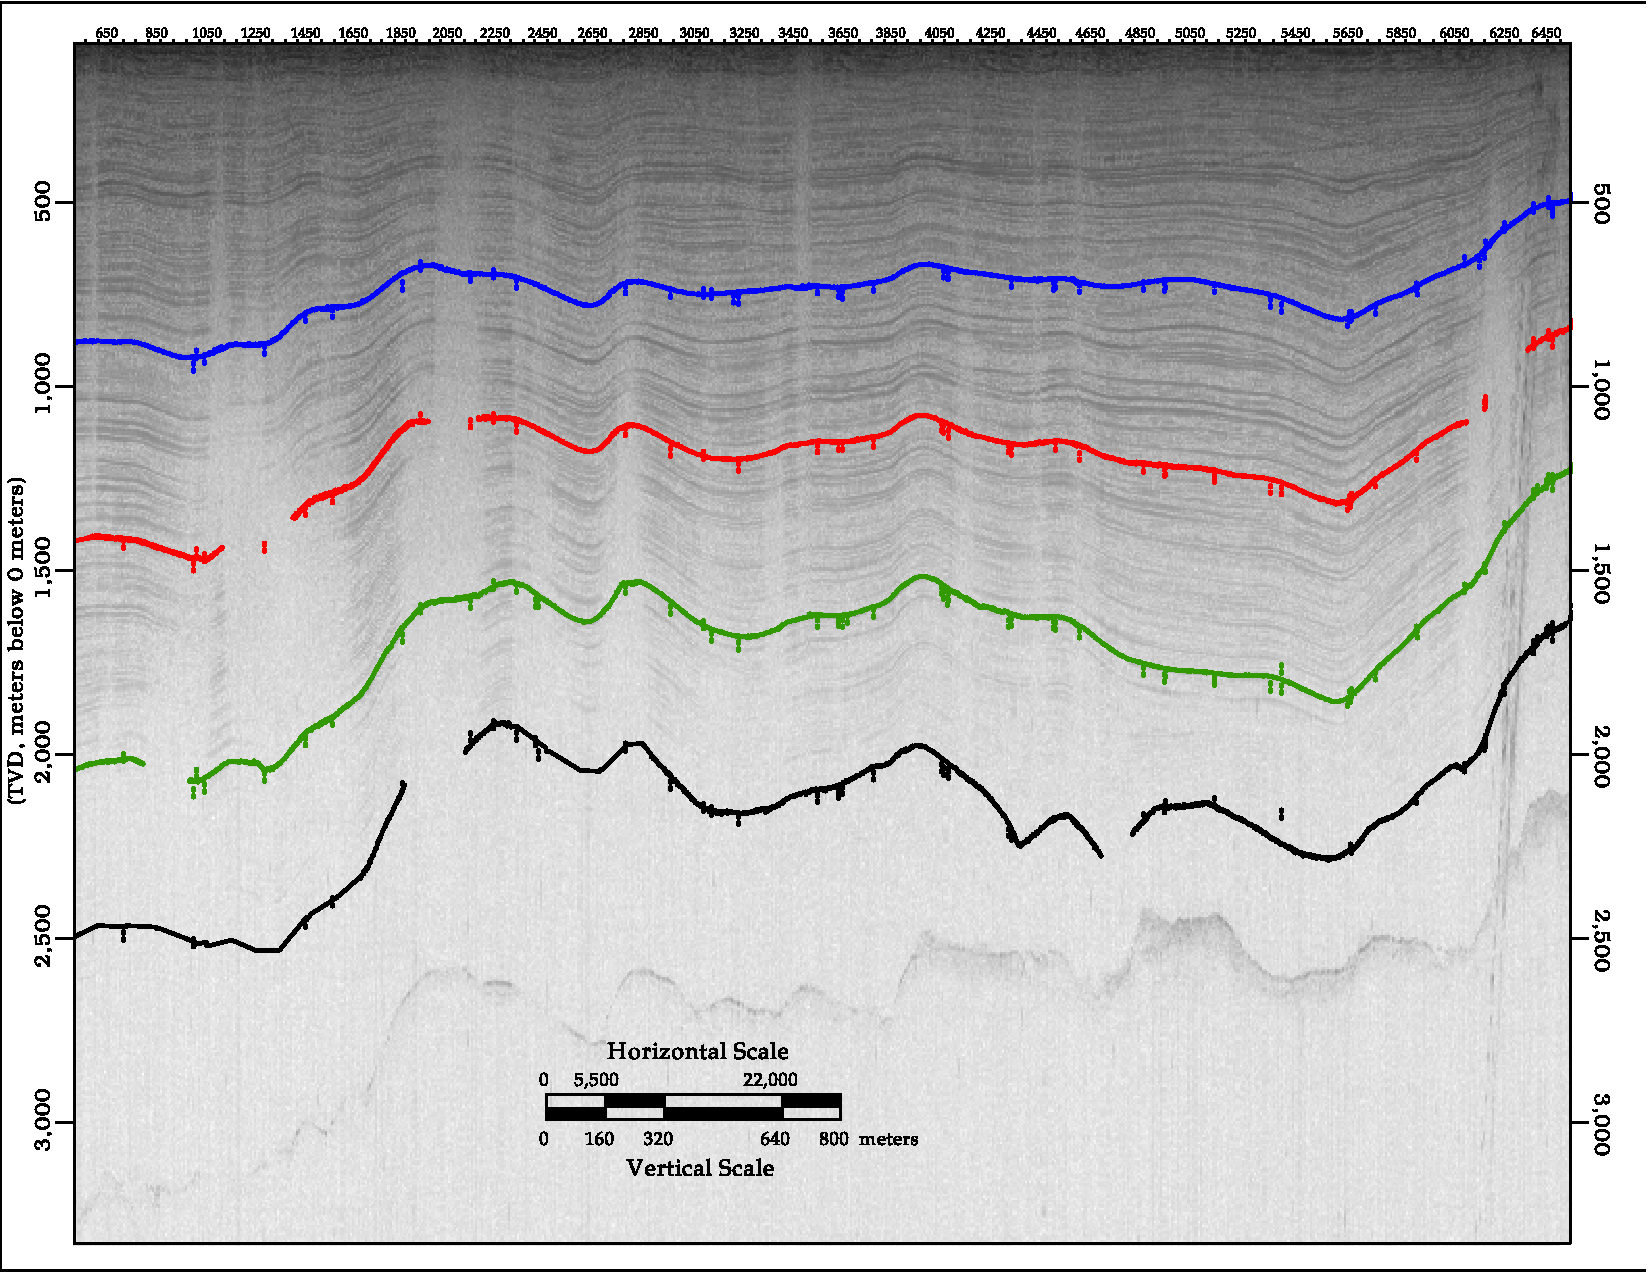
\includegraphics[scale=0.6]{/Users/gail/Documents/Research/Projects/Layers/paper/figures/radargram-4layers-paper}}
%\captionsetup{width=.9\textwidth}
\caption{Radargram showing reflectors of interest near the Byrd ice core along flight line ICP6/MKB2l/F14T01a observed using the HiCARS2 radar system. Short vertical hatches along tracked reflectors show intersections with crosslines.}
\label{fig:layergram}
\end{figure}


To estimate reflector depths from TWTT ($TWTT_{m,r}(D_r)$), we use a simple relation between the different velocities of the radar signal in air and in ice and incorporate several known sources of uncertainty, including: 1) variations in the radar velocity in ice due to ice temperature and fabric ($v_{ice}$), 2) vertical precision limitations of radar range detection ($\sigma_{prec}$), and 3) uncertainty in the firn correction ($\epsilon_{firn}$) due to measurement errors in the ice density profile:

\begin{equation}\label{deptheqn}
%D_r= \frac{1}{2}[(TWTT_r + \epsilon_{prec,r}) - (TWTT_{surf} + \epsilon_{prec,surf})] \cdot v_{ice} + d_{firn}\\
TWTT_{m,r}(D_r) + \sigma_{prec,r} = 2 \frac{D_r - (d_{firn}+\epsilon_{firn})}{v_{ice}} + (TWTT_{surf} + \epsilon_{prec,surf})
\end{equation}

The complexity of local ice properties affecting the velocity at any location and depth make it difficult to know the true velocity. Empirical evidence suggests a range of expected velocities and we conservatively assume they are uniformly distributed such that: $p(v_{ice}) ~\sim U[168,169.5]\,m/{\mu}s$ \citep{fujita2000}. In lieu of detailed observations of ice properties with depth, we assume the value of $v_{ice}$ is a constant throughout the ice column and apply it systematically to all reflector depths.

The radar pulse width determines vertical precision, $\sigma_{prec,r}$ \citep{millar1982}. We assume a finite pulse width, meaning an infinitesimally thin layer of ice will appear in the survey to have a finite width. This can lead to errors in tracing isochronous reflectors, as the reflected energy from a finite depth will include ice with a range of ages. To account for this, we include uncertainty due to range precision, according to the signal to noise ratio of each reflector's radar amplitude as in \citet{cavitte2016}:

\begin{equation}
\sigma_{prec,r} = \frac{\Delta{r}}{\sqrt{SNR_r}}
\end{equation} 
The range resolution, $\Delta{r}$, is 8.4 m for all reflectors in the HiCARS2 system \citep{young2011}. Values of the SNR for each reflector are shown in Table~\ref{tab:depthunc}. 

%We assume this error is normal such that $p(\epsilon_{prec}) = N(0,\sigma_r)$ ns. Values of $\epsilon_{prec}$ are sampled for each reflector independently.

Finally, a firn layer with variable density \citep{gow1970} exists in the upper part of the ice sheet. The velocity of the radar is faster in firn than in solid ice. To correct for the underestimation of ice depth if the firn layer is not considered, we estimate the firn correction ($d_{firn}$), the difference between the ice thickness with and without the firn layer present . %Based on the density profile and firn thickness ($\sim$ 65 m) at the Byrd ice core site \citep{gow1970}, we estimate the prior on $d_{firn}$ to be $p(d_{firn})\sim$ U[6, 36]\,m. This assumes firn density ranges from 400 - 8030 $\frac{kg}{m^3}$ and glacial ice ranges from 830 - 917 $\frac{kg}{m^3}$ \citep{paterson1994}. The firn correction is applied to all estimates of englacial reflector depth in this study because they are all deeper than the measured firn layer.
Errors in density, $\rho(z)$, are used to estimate the error in $d_{firn}$, $\epsilon_{firn}$. These errors are known for the WAIS Divide measurements, but not for the Byrd ice core profile. In lieu of density measurement errors at the Byrd site, we assume the errors to be consistent with those observed at the WAIS Divide ice core. These errors are assumed gaussian, randomly sampled, and the firn correction is computed using the \citet{dowdeswell2004} relation:

\begin{equation}
d_{firn} = \frac{K}{n^{'}_{i}}\int{(\rho_{i} - \rho(z)) dz}
\end{equation}
where K is 0.85 m$^{3}$ Mg$^{-1}$ \citep{robin1969}, $n^{'}_{i}$ is the refractive index of ice ($n^{'}_{i}$=1.78), $\rho_{i}$ is the density of ice ($\rho_{i}$=0.917 Mg m$^{-3}$) and $\rho(z)$ is the density of ice at depth \textit{z} with units Mg m$^{-3}$.

The TWTT from the observing aircraft to the surface of the ice sheet is known from interpretation of the surface reflector, $TWTT_{surf}$. The computed depth of each reflector is relative to this surface reflector. Just as each reflector may have TWTT precision errors independent of the others, errors in the distance between the surface and the acquisition aircraft are common to all observed reflectors in the ice column. Therefore, a randomly sampled precision error, $\epsilon_{prec,surf}$, is applied systematically to all reflectors.







\label{radardepth}
\subsection{Metropolis Algorithm}\label{metrop}
At each iteration, the Metropolis/Gibbs sampling algorithm \citep{metropolis1953,hastings1970} proposes values for parameters of interest (those with priors in Equation~\ref{eqn:bigproblem}). The algorithm accepts or rejects proposed sets of parameter values by comparison between the proposed and previously-accepted likelihood (or ``cost") values. A low cost value represents good agreement between model and observations, reflecting a small model-data misfit. According to the Metropolis/Gibbs algorithm, if the cost associated with proposed parameters is lower than that of the last accepted iteration, the proposed parameter values are accepted. Alternatively, higher cost values may be accepted with a probability determined by the likelihood. Each likelihood function is considered separately and both must represent an adequate solution on a given iteration for the proposed parameters to be accepted.


There are two likelihood functions, describing the model-data misfit between reflector depth and age, respectively:


\begin{equation}\label{eqn:loglikeage}
p(A_{IC} | D_{IC},\vec{f},S) \propto exp[\frac{-S\sum_{j = 61}[A_{IC,j} - A_{m,j}(\vec{f},D_{IC})]^2}{2\sigma_A^2} + r^6]
\end{equation}

\begin{equation}\label{eqn:loglikedepth}
p(TWTT_r | D_r,d_{firn},v_{ice} ) \propto exp[\frac{-\sum_{i=4}[TWTT_{r,i} - TWTT_{m,i}(D_r)]^2}{2\sigma_{TWTT}^2}]
\end{equation}


In the depth likelihood function, $TWTT_m(D_r)$ is based on the relationship between depth and TWTT as in Equation~\ref{deptheqn} and $TWTT_r$ is observed by ice-penetrating radar for each reflector, $i$. To estimate $\sigma_{TWTT}$, we assume a perfect model and compute with standard deviation of the numerator given typical errors we expect affect our data. This method allows for correlation between depth errors, as expected. More details are discussed in the Supplement.


In the age likelihood function, the modeled age, $A_m$, is a function of ice flow model parameters, $\vec{f}$. A regularization term, $r^6$, is used to penalize large variability in the sampled accumulation rate function input to the ice flow model and $A_m$ comes from solutions to the forward ice flow model. We train our model on $J=61$ volcanic events from \citet{hammer1997}. Importantly, these volcanic ages are overly confident in that they do not include uncertainty information. To accomodate additional unknown uncertainty in this data, we include an unknown precision parameter, $S$, and use it to infer uncertainty in the volcanic record from scatter between our model and the observed data. $S$ is a ``nuisance" parameter that accounts for uncertainty in $\sigma_A$ by using $E_m$ as a measure of scatter between modeled age $A_m$ and $\Pi(S) \propto Ga(\alpha,\beta)$ The posterior probability distribution of $S$ is therefore:

\begin{equation}\label{eqn:S}
PPD(S) = Ga(\frac{k_e}{2}+\alpha, E_m+\beta)
\end{equation}
where 
\begin{equation}
 E_m= \frac{\sum_{j}[A_{IC,j} - A_{m,j}(\vec{f},D_{IC})]^2}{2\sigma_A^2} 
\end{equation}

Parameters $\alpha$ and $\beta$ are assumed to be 1 as in the case for a noninformative gamma prior. The scatter between the model and data is represented by the cost, $E_m$, which determines the uncertainty. The number of degrees of freedom, $k_e$, is assumed to be less than $J$ due to covariation in the age and depth of ice. Because we do not know the value of $k_e$ a priori, we assume $k_e = \frac{J}{2}$ (see Supplement). Unlike other parameters in our problem in which Metropolis-Hastings sampling is used, values of $S$ are proposed using Gibbs sampling \citep{gelfand1992}, effectively estimating reflector age uncertainty given the choice of parameter solution for each iteration.


%The Metropolis algorithm randomly samples each of the ice flow parameters and computes an age-depth profile. A Bayesian method is used to determine suitability of proposed ice flow parameters in a Bayesian way:
%\begin{equation}\label{posterior}
% p(\vec{f},\sigma_V | A_V, D_V) \propto p(A_V,D_V | \vec{f},\sigma_V) p(\vec{f}) p(\sigma_V),
%\end{equation}
%A posterior probability, $p(A | \vec{f})$, is computed for each set of parameters from likelihood and prior probabilities, $P(\vec{f})$. As described below, we require only the proportional relation because relative posterior values are considered in this Markov Chain process.

%The simulated age-depth profile is compared to the observed volcanic chronology using the ``log-likelihood" function, $p(A_V,D_V | \vec{f},\sigma_V)$, to quantify how closely a sampled set of parameters represents the observed ice profile:
%
%\begin{equation}\label{cost}
%ln(likelihood) = \frac{1}{N}\sum\frac{(A_{sim}(\vec{f})_i~ - ~A_{V,i})^2}{(2\sigma_{V})^2},
%\end{equation}
%where $\vec{Age}_{sim}$ comes from evaluating the ice flow model for parameter values sampled from $\vec{f}$. $A_{V}$ and $\sigma_{V}$ describe the observed volcanic chronology at the Byrd ice core. The prior on $\sigma_{V}$ is 
%\begin{equation}
%p(\sigma_V) \sim Ga(\alpha, \beta)
%\end{equation}

%which assumes error in the chronology is $\sim$3\% (T.J. Fudge, pers. comm.). Uncertainty in the volcanic chronology, $\sigma_{V}$, loosens the constraint on how closely $A_{sim}$ must match $A_{V}$ to be acceptable. We assume $N$ degrees of freedom, where $N$ is the number of volcanic observations. This is because observed global volcanic events are assumed independent.
%



%\subsubsection{Estimating accumulation}\label{accum}
The accumulation rate, $\dot{a}$, is highly uncertain for the Byrd ice core, so we compare ice flow model solutions using several accumulation functions. These include constant accumulation, a theoretical function derived for an expected atmospheric temperature timeseries at the nearby WAIS Divide ice core\citet{morse2002}, constant accumulation rates every 5,000 years, and constant accumulation rates in four depth bins which correspond to observed changes in layer thickness at the byrd ice core \citep{}. \textbf{Adding an accumulation function based on Byrd ice core isotopes.}

The result is shown in Figure \ref{fig:accumfunc}. We see that \textbf{One of them does better than the others. This one will be used in the final model to give the real result of age-depth for all the reflectors.}


%\begin{figure}
%%\begin{center}
%\centering
%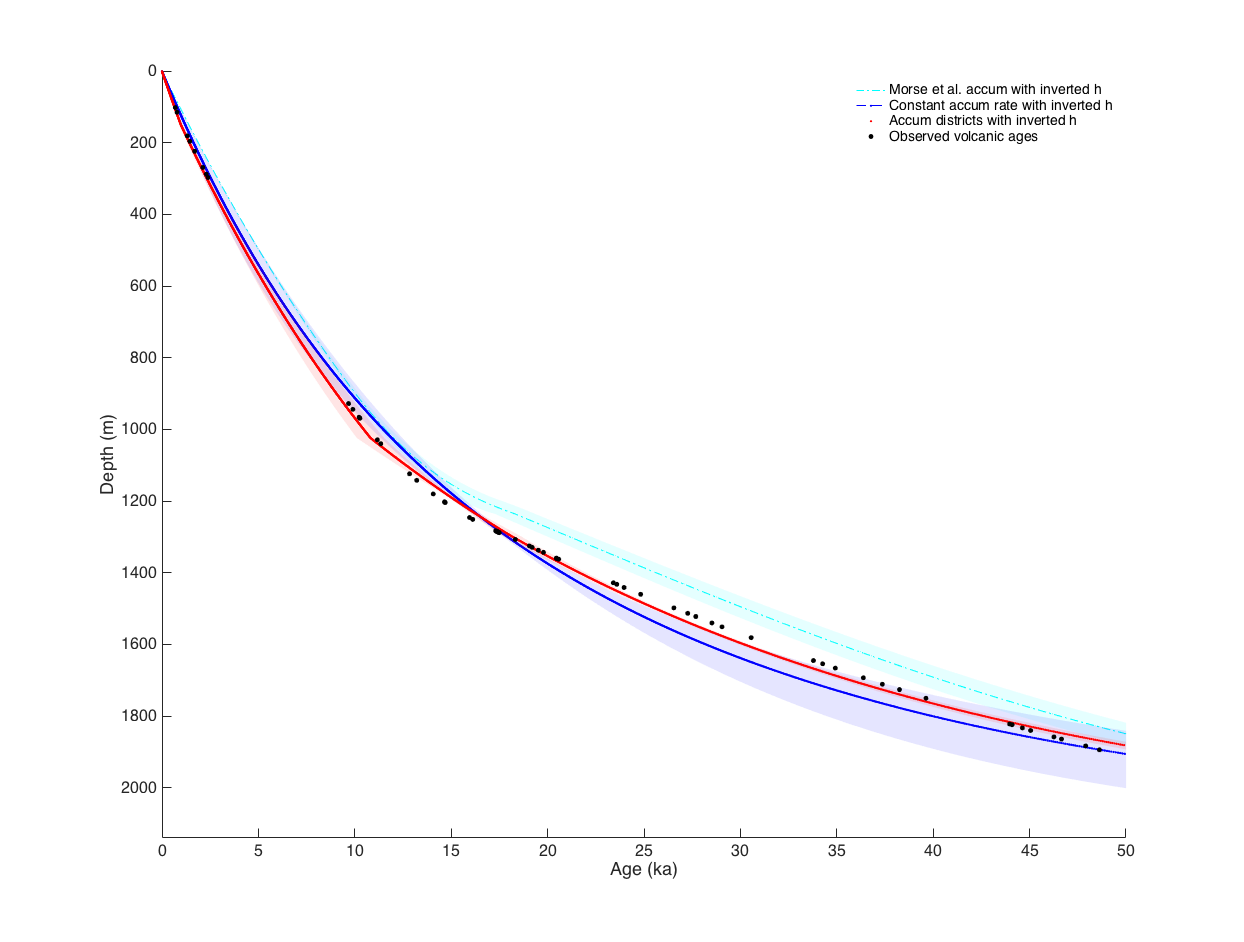
\includegraphics[scale=0.4]{figures/accumfunc}
%%\captionsetup{width=.9\textwidth}
%\caption[]{\textbf{Unfortunately, this figure is missing the 5k year interval which is the best (but takes the longest to run). In general, the accumulation functions fit the volcanic data well, but perhaps too well as seen in the comparison with the WAIS Divide ice core. This is a proof of concept that the data can be modeled using the MCMC method and we therefore can compute an age-depth profile even where there is no data, but the uncertainty so far is being underestimated.}}
%%\end{center}
%\label{fig:accumfunc}
%\end{figure}




	\subsubsection{Ice flow model at the Byrd ice core}
%This is consistent with experiment opinion that ice core age uncertainty is generally 2-3$\%$ of ice age (T.J. Fudge, private communication). Therefore, we construct an age-depth distribution for the Byrd ice core using statistical methods and an assumed 3$\%$ age uncertainty. The derived age-depth profile is then compared to the WAIS Divide profile using englacial layers that have been tracked between the two ice core sites. 

Due to the inherent stratigraphic dependence of age in the ice column, we use a flow model to simulate the age-depth relationship. We use a simple, one-dimensional model of ice flow (Equation \ref{schwander}) which derives ice age from accumulation and strain rate, assuming constant horizontal strain rate in the upper part of the ice sheet and a shear layer of thickness $h$ at the bottom of the ice sheet, for which we invert \citep{schwander2001}. In the shear layer, the strain rate is assumed to decrease linearly and the bottom of the ice is assumed sliding with velocity $q$ $\cdot$ $v_0$, where $v_0$ is the horizontal velocity at the surface.

\begin{equation}\label{schwander}
A(z) = \int_{z}^{H} \frac{dz}{\epsilon_z \dot{a}(z)}
\end{equation}
where
\begin{center}
$    \epsilon_z=
    \begin{cases}
                 1-k(H-z), & h \leq z \leq H \\
                  kz(q+\frac{1-q}{2h}z), & 0 < z < h
    \end{cases}, 
$
$
k = \frac{2}{2H - h(1-q)}
$
\end{center}
$H$ is ice thickness in ice equivalent, $z$ is height above the bed, $h$ is the depth to the shear layer, $\dot{a}$ is the layer thickness, and $q$ is a constant for which we invert. 

The ice flow model accounts for two primary factors in the age-depth profile: burial as a function of accumulation rate, $\dot{a}$, and thinning as a function of strain, $\epsilon_z$. In the simplest realization, ice deposited at a given time at the ice sheet surface will be found at a depth in the ice sheet corresponding to the amount of subsequent accumulation. However, due to strain thinning at depth, the ice will be less deep than would be expected if accumulation alone is considered. 

In Section~\ref{metrop}, we invert for the flow parameters $h$, $q$, and $\dot{a}$. Constant values for $h$ and $q$ are sampled from uniform priors defined in a conservative range. Accumulation is estimated for 11 units of depth spaced every 200 m starting from the ice surface and are sampled from the same uniform prior.

\begin{center}
%\begin{equation}
$p(\vec{f}) = 
	\begin{cases}
		p(h) \sim U(0, 0.5) \\
		p(q) \sim U (0, 1) \\
		p(\dot{a}_{z < 200 m ... z > 2000 m}) \sim U(0.5~m/a,0.15~m/a)\\
	\end{cases}
$	
%\end{equation}	
\end{center}

The prior distributions of flow parameters, together denoted as $p(\vec{f})$, assume the shear layer is in the bottom half of the ice sheet depth and that the bed of the ice sheet is moving slower than the surface. Accumulation as a function of depth, $\dot{a}$, is sampled from 11 distinct depth bins spanning the ice thickness. This allows for variability of accumulation over time, as expected. To limit unrealistic variability in accumulation between depth bins, Tikhonov regularization is used on the age likelihood function to punish estimates of the accumulation function which are highly-variable relative to a solution computed with no regularization and smoothed over a moving 600-m depth window.

	


\subsection{Radar depth and error model}
 Radar pulses transmitted into the ice sheet reflect off surfaces of dielectric contrast in the ice that are the result of variations in ice fabric, composition, temperature, and rheology of ice \citep{fujita2000}. The reflected signal is received by the radar system and recorded as two-way travel time (TWTT) from transmission to receipt.  The reflector data in this analysis (Figure~\ref{fig:layergram}) were collected by the University of Texas Institute for Geophysics, including GIMBLE \citep{gimble2017}, AGASEA \citep{holt2006}, CASERTZ \citep{morse2002}, and SOAR/WMB \citep{luyendyk2003} (Figure~\ref{fig:radarmap}). Data used to trace reflectors between Byrd ice core and WAIS Divide ice core were collected from a DC-3 or Twin Otter airborne platform and used the HiCARS coherent radar system with 60 MHz center frequency and 15 MHz bandwidth \citep{peters2005}.% or the TUD-derived incoherent radar sounder \citep{blankenship2001} with 4 MHz bandwidth.

\begin{figure}[h]
\centering
\makebox[\textwidth][c]{
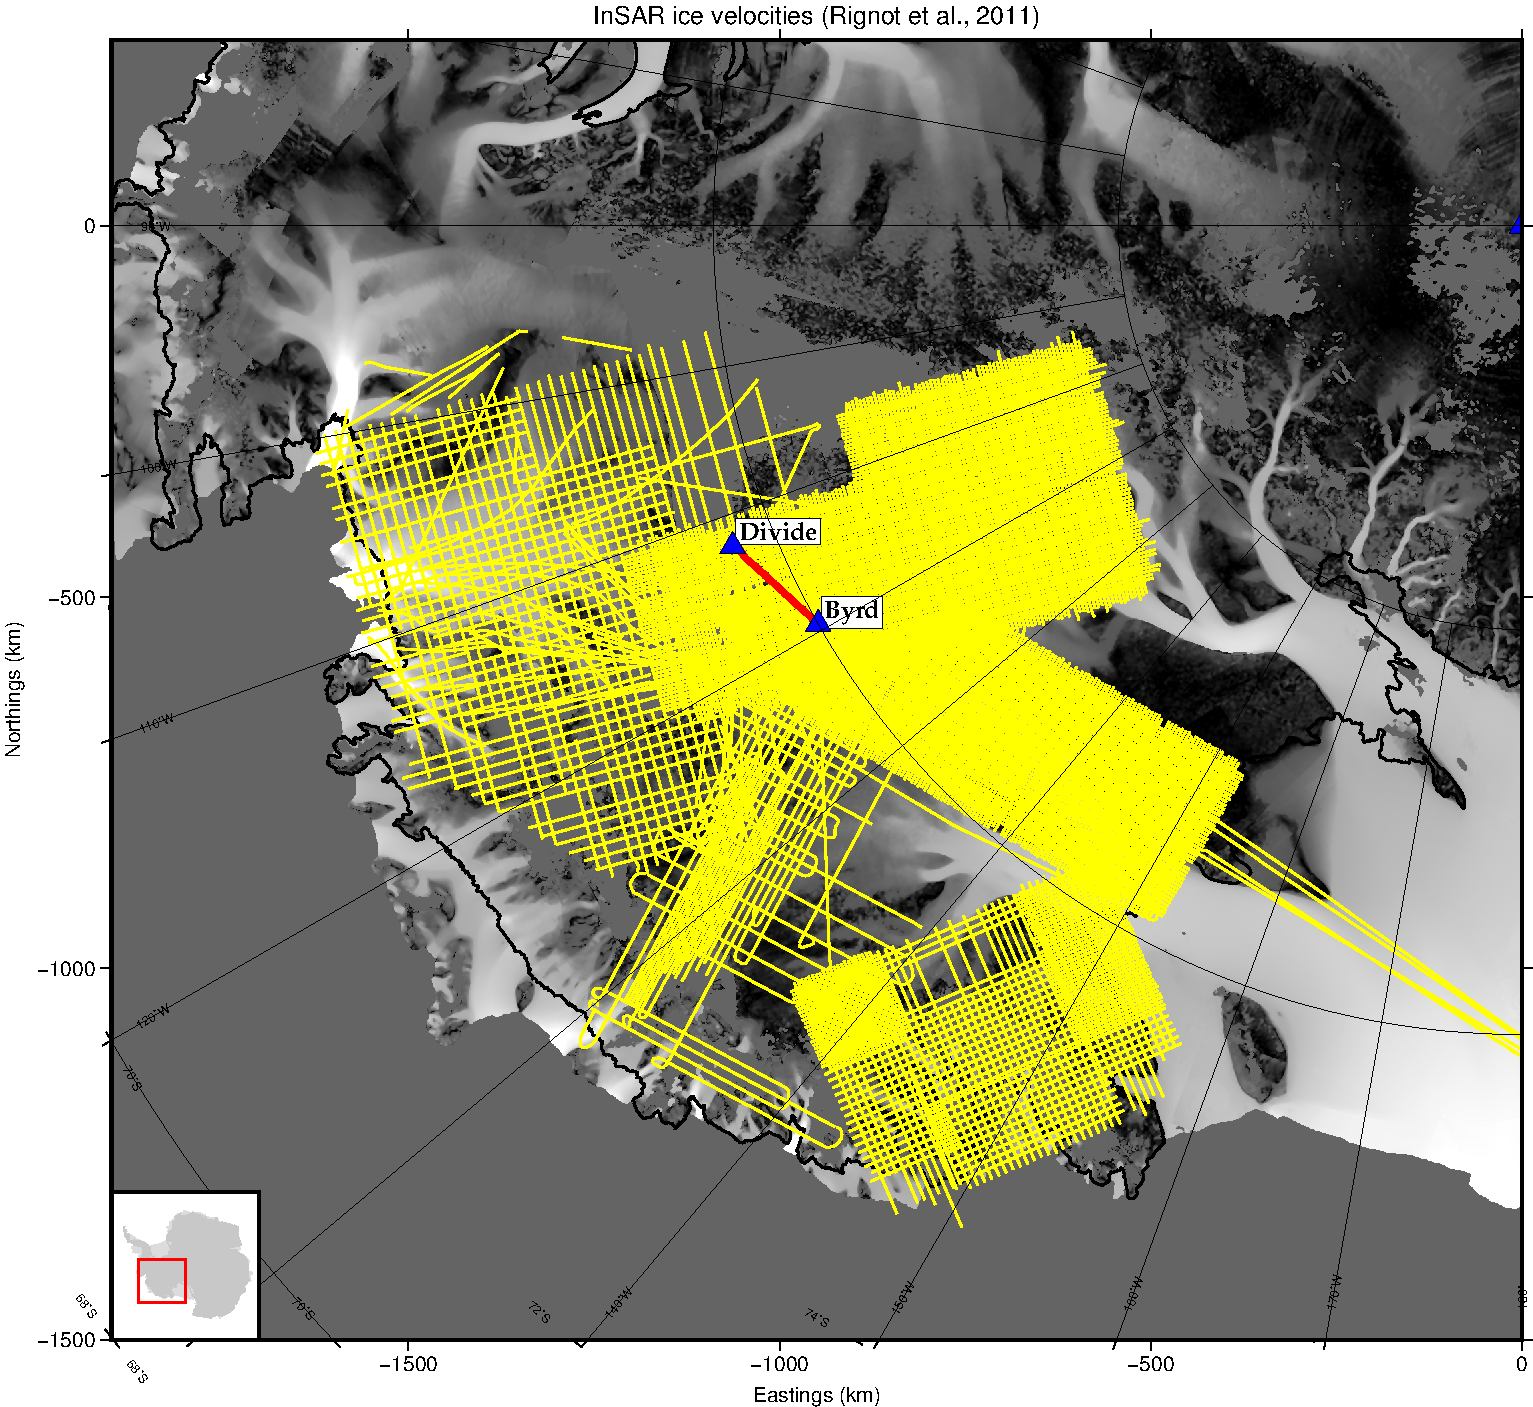
\includegraphics[scale=0.5]{/Users/gail/Documents/Research/Projects/Layers/analysis/figures/WAIS_vel_gray_final}}
%\captionsetup{width=.9\textwidth}
\caption{Map of central West Antarctic with available airborne geophysical radar surveys (yellow lines) and  WAIS Divide and Byrd ice core locations (blue triangles) overlain. Gray shading is surface velocity \citep{rignot2011}. The red line denotes the flight line along which the reflectors in this study were observed. }
\label{fig:radarmap}
\end{figure}



In this study, we consider TWTT of four reflectors spanning the ice thickness in the region of central West Antarctica (Figure~\ref{fig:layergram}). These reflectors have been tracked using Halliburton's Landmark seismic interpretation software and can be tied to both the Byrd and WAIS Divide ice cores for dating using observations from the HiCARS system (Figure~\ref{fig:radarmap}). %Determining the depth of the reflectors, $D_r$, may be affected by several sources of uncertainty, including uncertainty in the firn depth, the velocity of the radar pulse in ice, and the pulse-limited precision of radar observations.

\begin{figure}[h]
\centering
\makebox[\textwidth][c]{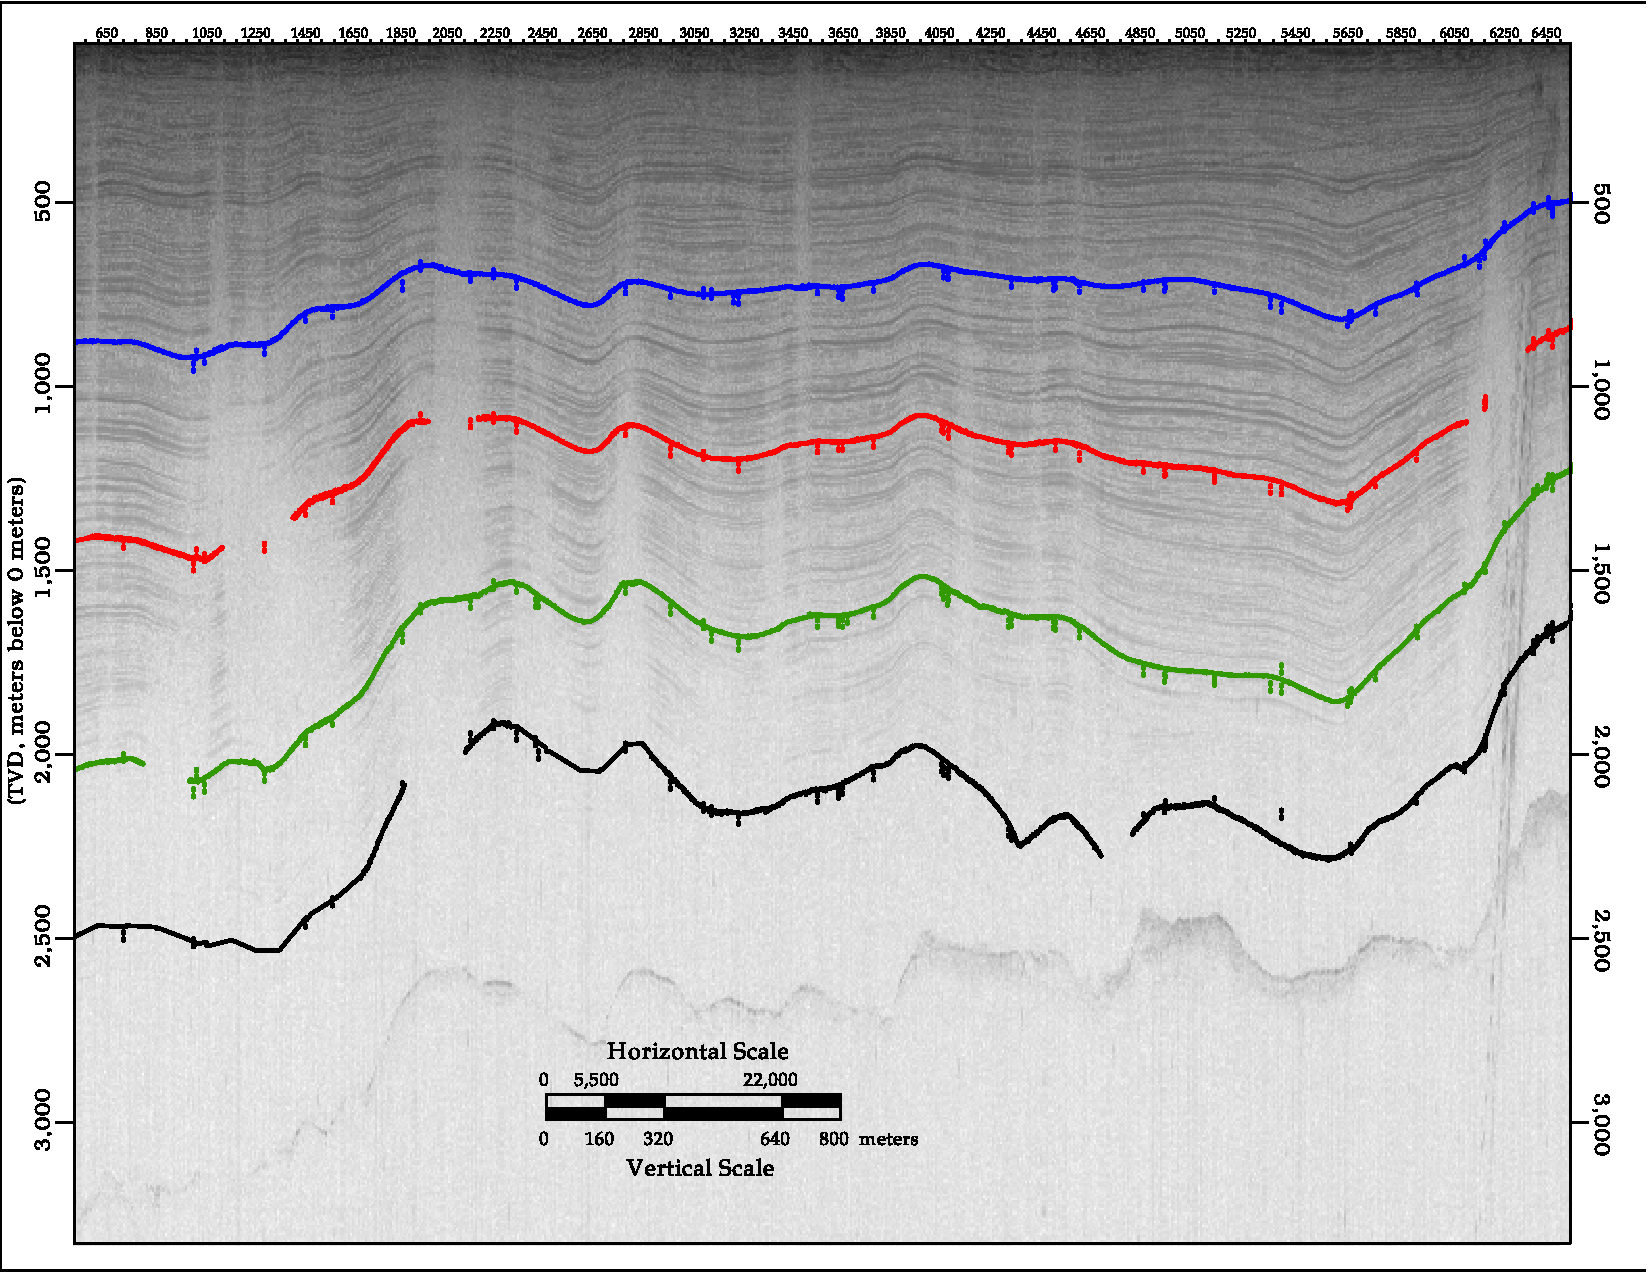
\includegraphics[scale=0.6]{/Users/gail/Documents/Research/Projects/Layers/paper/figures/radargram-4layers-paper}}
%\captionsetup{width=.9\textwidth}
\caption{Radargram showing reflectors of interest near the Byrd ice core along flight line ICP6/MKB2l/F14T01a observed using the HiCARS2 radar system. Short vertical hatches along tracked reflectors show intersections with crosslines.}
\label{fig:layergram}
\end{figure}


To estimate reflector depths from TWTT ($TWTT_{m,r}(D_r)$), we use a simple relation between the different velocities of the radar signal in air and in ice and incorporate several known sources of uncertainty, including: 1) variations in the radar velocity in ice due to ice temperature and fabric ($v_{ice}$), 2) vertical precision limitations of radar range detection ($\sigma_{prec}$), and 3) uncertainty in the firn correction ($\epsilon_{firn}$) due to measurement errors in the ice density profile:

\begin{equation}\label{deptheqn}
%D_r= \frac{1}{2}[(TWTT_r + \epsilon_{prec,r}) - (TWTT_{surf} + \epsilon_{prec,surf})] \cdot v_{ice} + d_{firn}\\
TWTT_{m,r}(D_r) + \sigma_{prec,r} = 2 \frac{D_r - (d_{firn}+\epsilon_{firn})}{v_{ice}} + (TWTT_{surf} + \epsilon_{prec,surf})
\end{equation}

The complexity of local ice properties affecting the velocity at any location and depth make it difficult to know the true velocity. Empirical evidence suggests a range of expected velocities and we conservatively assume they are uniformly distributed such that: $p(v_{ice}) ~\sim U[168,169.5]\,m/{\mu}s$ \citep{fujita2000}. In lieu of detailed observations of ice properties with depth, we assume the value of $v_{ice}$ is a constant throughout the ice column and apply it systematically to all reflector depths.

The radar pulse width determines vertical precision, $\sigma_{prec,r}$ \citep{millar1982}. We assume a finite pulse width, meaning an infinitesimally thin layer of ice will appear in the survey to have a finite width. This can lead to errors in tracing isochronous reflectors, as the reflected energy from a finite depth will include ice with a range of ages. To account for this, we include uncertainty due to range precision, according to the signal to noise ratio of each reflector's radar amplitude as in \citet{cavitte2016}:

\begin{equation}
\sigma_{prec,r} = \frac{\Delta{r}}{\sqrt{SNR_r}}
\end{equation} 
The range resolution, $\Delta{r}$, is 8.4 m for all reflectors in the HiCARS2 system \citep{young2011}. Values of the SNR for each reflector are shown in Table~\ref{tab:depthunc}. 

%We assume this error is normal such that $p(\epsilon_{prec}) = N(0,\sigma_r)$ ns. Values of $\epsilon_{prec}$ are sampled for each reflector independently.

Finally, a firn layer with variable density \citep{gow1970} exists in the upper part of the ice sheet. The velocity of the radar is faster in firn than in solid ice. To correct for the underestimation of ice depth if the firn layer is not considered, we estimate the firn correction ($d_{firn}$), the difference between the ice thickness with and without the firn layer present . %Based on the density profile and firn thickness ($\sim$ 65 m) at the Byrd ice core site \citep{gow1970}, we estimate the prior on $d_{firn}$ to be $p(d_{firn})\sim$ U[6, 36]\,m. This assumes firn density ranges from 400 - 8030 $\frac{kg}{m^3}$ and glacial ice ranges from 830 - 917 $\frac{kg}{m^3}$ \citep{paterson1994}. The firn correction is applied to all estimates of englacial reflector depth in this study because they are all deeper than the measured firn layer.
Errors in density, $\rho(z)$, are used to estimate the error in $d_{firn}$, $\epsilon_{firn}$. These errors are known for the WAIS Divide measurements, but not for the Byrd ice core profile. In lieu of density measurement errors at the Byrd site, we assume the errors to be consistent with those observed at the WAIS Divide ice core. These errors are assumed gaussian, randomly sampled, and the firn correction is computed using the \citet{dowdeswell2004} relation:

\begin{equation}
d_{firn} = \frac{K}{n^{'}_{i}}\int{(\rho_{i} - \rho(z)) dz}
\end{equation}
where K is 0.85 m$^{3}$ Mg$^{-1}$ \citep{robin1969}, $n^{'}_{i}$ is the refractive index of ice ($n^{'}_{i}$=1.78), $\rho_{i}$ is the density of ice ($\rho_{i}$=0.917 Mg m$^{-3}$) and $\rho(z)$ is the density of ice at depth \textit{z} with units Mg m$^{-3}$.

The TWTT from the observing aircraft to the surface of the ice sheet is known from interpretation of the surface reflector, $TWTT_{surf}$. The computed depth of each reflector is relative to this surface reflector. Just as each reflector may have TWTT precision errors independent of the others, errors in the distance between the surface and the acquisition aircraft are common to all observed reflectors in the ice column. Therefore, a randomly sampled precision error, $\epsilon_{prec,surf}$, is applied systematically to all reflectors.







\label{radardepth}
	\subsection{Metropolis Algorithm}\label{metrop}
At each iteration, the Metropolis/Gibbs sampling algorithm \citep{metropolis1953,hastings1970} proposes values for parameters of interest (those with priors in Equation~\ref{eqn:bigproblem}). The algorithm accepts or rejects proposed sets of parameter values by comparison between the proposed and previously-accepted likelihood (or ``cost") values. A low cost value represents good agreement between model and observations, reflecting a small model-data misfit. According to the Metropolis/Gibbs algorithm, if the cost associated with proposed parameters is lower than that of the last accepted iteration, the proposed parameter values are accepted. Alternatively, higher cost values may be accepted with a probability determined by the likelihood. Each likelihood function is considered separately and both must represent an adequate solution on a given iteration for the proposed parameters to be accepted.


There are two likelihood functions, describing the model-data misfit between reflector depth and age, respectively:


\begin{equation}\label{eqn:loglikeage}
p(A_{IC} | D_{IC},\vec{f},S) \propto exp[\frac{-S\sum_{j = 61}[A_{IC,j} - A_{m,j}(\vec{f},D_{IC})]^2}{2\sigma_A^2} + r^6]
\end{equation}

\begin{equation}\label{eqn:loglikedepth}
p(TWTT_r | D_r,d_{firn},v_{ice} ) \propto exp[\frac{-\sum_{i=4}[TWTT_{r,i} - TWTT_{m,i}(D_r)]^2}{2\sigma_{TWTT}^2}]
\end{equation}


In the depth likelihood function, $TWTT_m(D_r)$ is based on the relationship between depth and TWTT as in Equation~\ref{deptheqn} and $TWTT_r$ is observed by ice-penetrating radar for each reflector, $i$. To estimate $\sigma_{TWTT}$, we assume a perfect model and compute with standard deviation of the numerator given typical errors we expect affect our data. This method allows for correlation between depth errors, as expected. More details are discussed in the Supplement.


In the age likelihood function, the modeled age, $A_m$, is a function of ice flow model parameters, $\vec{f}$. A regularization term, $r^6$, is used to penalize large variability in the sampled accumulation rate function input to the ice flow model and $A_m$ comes from solutions to the forward ice flow model. We train our model on $J=61$ volcanic events from \citet{hammer1997}. Importantly, these volcanic ages are overly confident in that they do not include uncertainty information. To accomodate additional unknown uncertainty in this data, we include an unknown precision parameter, $S$, and use it to infer uncertainty in the volcanic record from scatter between our model and the observed data. $S$ is a ``nuisance" parameter that accounts for uncertainty in $\sigma_A$ by using $E_m$ as a measure of scatter between modeled age $A_m$ and $\Pi(S) \propto Ga(\alpha,\beta)$ The posterior probability distribution of $S$ is therefore:

\begin{equation}\label{eqn:S}
PPD(S) = Ga(\frac{k_e}{2}+\alpha, E_m+\beta)
\end{equation}
where 
\begin{equation}
 E_m= \frac{\sum_{j}[A_{IC,j} - A_{m,j}(\vec{f},D_{IC})]^2}{2\sigma_A^2} 
\end{equation}

Parameters $\alpha$ and $\beta$ are assumed to be 1 as in the case for a noninformative gamma prior. The scatter between the model and data is represented by the cost, $E_m$, which determines the uncertainty. The number of degrees of freedom, $k_e$, is assumed to be less than $J$ due to covariation in the age and depth of ice. Because we do not know the value of $k_e$ a priori, we assume $k_e = \frac{J}{2}$ (see Supplement). Unlike other parameters in our problem in which Metropolis-Hastings sampling is used, values of $S$ are proposed using Gibbs sampling \citep{gelfand1992}, effectively estimating reflector age uncertainty given the choice of parameter solution for each iteration.


%The Metropolis algorithm randomly samples each of the ice flow parameters and computes an age-depth profile. A Bayesian method is used to determine suitability of proposed ice flow parameters in a Bayesian way:
%\begin{equation}\label{posterior}
% p(\vec{f},\sigma_V | A_V, D_V) \propto p(A_V,D_V | \vec{f},\sigma_V) p(\vec{f}) p(\sigma_V),
%\end{equation}
%A posterior probability, $p(A | \vec{f})$, is computed for each set of parameters from likelihood and prior probabilities, $P(\vec{f})$. As described below, we require only the proportional relation because relative posterior values are considered in this Markov Chain process.

%The simulated age-depth profile is compared to the observed volcanic chronology using the ``log-likelihood" function, $p(A_V,D_V | \vec{f},\sigma_V)$, to quantify how closely a sampled set of parameters represents the observed ice profile:
%
%\begin{equation}\label{cost}
%ln(likelihood) = \frac{1}{N}\sum\frac{(A_{sim}(\vec{f})_i~ - ~A_{V,i})^2}{(2\sigma_{V})^2},
%\end{equation}
%where $\vec{Age}_{sim}$ comes from evaluating the ice flow model for parameter values sampled from $\vec{f}$. $A_{V}$ and $\sigma_{V}$ describe the observed volcanic chronology at the Byrd ice core. The prior on $\sigma_{V}$ is 
%\begin{equation}
%p(\sigma_V) \sim Ga(\alpha, \beta)
%\end{equation}

%which assumes error in the chronology is $\sim$3\% (T.J. Fudge, pers. comm.). Uncertainty in the volcanic chronology, $\sigma_{V}$, loosens the constraint on how closely $A_{sim}$ must match $A_{V}$ to be acceptable. We assume $N$ degrees of freedom, where $N$ is the number of volcanic observations. This is because observed global volcanic events are assumed independent.
%



	
\section{Dated englacial reflectors at the Byrd ice core}\label{agedepthresults}
	%\subsection{Updated Byrd ice core chronology}\label{agedepthresults}
%\textbf{The 5,000-year accumulation function gives the best fit of the volcanic observations at the Byrd ice core, so it is used in the final ice flow model effort. The resulting uncertainties in radar depth and age to each of the layers of interest in shown in Table~\ref{tab:depthunc}. For the deepest observed reflector that can be traced between WAIS Divide ice core and Byrd ice core, the depth and age uncertainty are 0.3\% and 5\%, respectively, at the 1$\sigma$ level. The mean and median ages and depths are consistent due to the gaussian nature of the errors, as shown in Figure~\ref{fig:layer_agedepth}.}

The age-depth distribution derived for the Byrd ice core site using these methods is shown in Figure~\ref{fig:spaghetti}. This updated chronology has been trained on previously-derived ECM estimates of volcanic events observed in the Byrd ice core, but also includes estimates of uncertainty in this data, radar observations, local ice flow parameters, and local accumulation rate. 

Corresponding probability density functions generated by the metropolis algorithm sample uncertainty in the age and depth for each of four radar reflectors observed near the Byrd ice core. The age of the observed reflectors increases dramatically with depth.  These observed reflectors span to before the Last Glacial Maximum, with the oldest and deepest observed reflector dated to 25.7 $\pm$ 1.82 ka. 

We assume radar reflectors to be isochronous such that their age should be the same whether observed at the Byrd ice core or the WAIS Divide ice core. To compare between the two ice cores, we use Halliburton's Landmark seismic interpreation software to track radar reflectors through central WAIS via existing flight lines shown in Figure~\ref{fig:radarmap}. We confirm the ages we compute for all four reflectors at the Byrd ice core site agree to within uncertainty with the independently-derived WAIS Divide ice core chronology (Figures~\ref{fig:layer_histo}b,c and ~\ref{fig:spaghetti}).

Estimated values of the model parameters can be seen in the Appendix. As expected, estimations of the depth of the four radar reflectors at each iteration (Figure~\ref{fig:depthconvergence}) are correlated to each other because knowledge of the depth and age of each layer informs the relative depth and age of all other reflectors. While the accumulation rate as a function of depth is unrealistically variable, our method includes a regularization term which takes into account the smoothed accumulation rate profile, as shown in Figure~\ref{fig:accumdepth}. The smoothed profiles more closely resemble a climatic record, for which the accumulation rate was lower during the Last Glacial Maximum% ($\sim$ 1400 m depth)
. 

%  %\begin{table}
%  \centering
%  \caption{ Depth and age mean, median, and uncertainty for ten strong radar reflectors near Byrd Station, West Antarctica. The radar two-way travel time (TWTT) is given in column 1. }
%  \begin{tabular}{ c c c c c c c}
%  \cline{1-7}
%  \multirow{2}{*}{Reflector} & TWTT& & Depth (m) & & Age  (a)& \\   
% % %& ($\mu$s)& Mean & Median & $\sigma$ & & Mean & Median & $\sigma$ \\
%  & ($\mu$s)& Mean  & $\sigma$ & &Mean  & $\sigma$ \\
%  \cline{3-4} \cline{6-7}
%   1 & 8.44    & 537.5  &  0.8 & &1200 & 20   \\
%   2 & 9.58    & 633.1  &  6.5 & &1770 & 40   \\
%   3 & 12.54   & 880.8  &  7.4 & &2100 & 60   \\
%   4 & 17.55   & 1300.7 &  6.1 & &3510 & 150  \\
%   5 & 22.42   & 1711.9 &  4.4 & &4360 & 200  \\
% %  %6 & 11.10  & 596.9  & 596.9  & 2.3 & &5440 & 5440 & 270   \\
% %  %7 & 12.78  & 738.8  & 738.8  & 2.3 & &7120 & 7110 & 370   \\
% %  %8 & 13.02  & 759.1  & 759.1  & 2.3 & 7350 & 7340 & 390   \\
% %  %9 & 18.92  & 1257.7 & 1257.7 & 2.4 & 16220 & 16300 & 1760   \\
% %  %10& 19.02  & 1266.2 & 1266.2 & 2.3 & 16400 & 16500 & 1820  \\
% % %\cline{1-7}
%  \end{tabular}
% % \tablenotetext{a}{Footnote text here.}
% % %\captionsetup{width=.9\textwidth}

%  %\label{tab:depthunc}
% %\end{table}




\begin{figure*}[h]
%\begin{center}
\centering
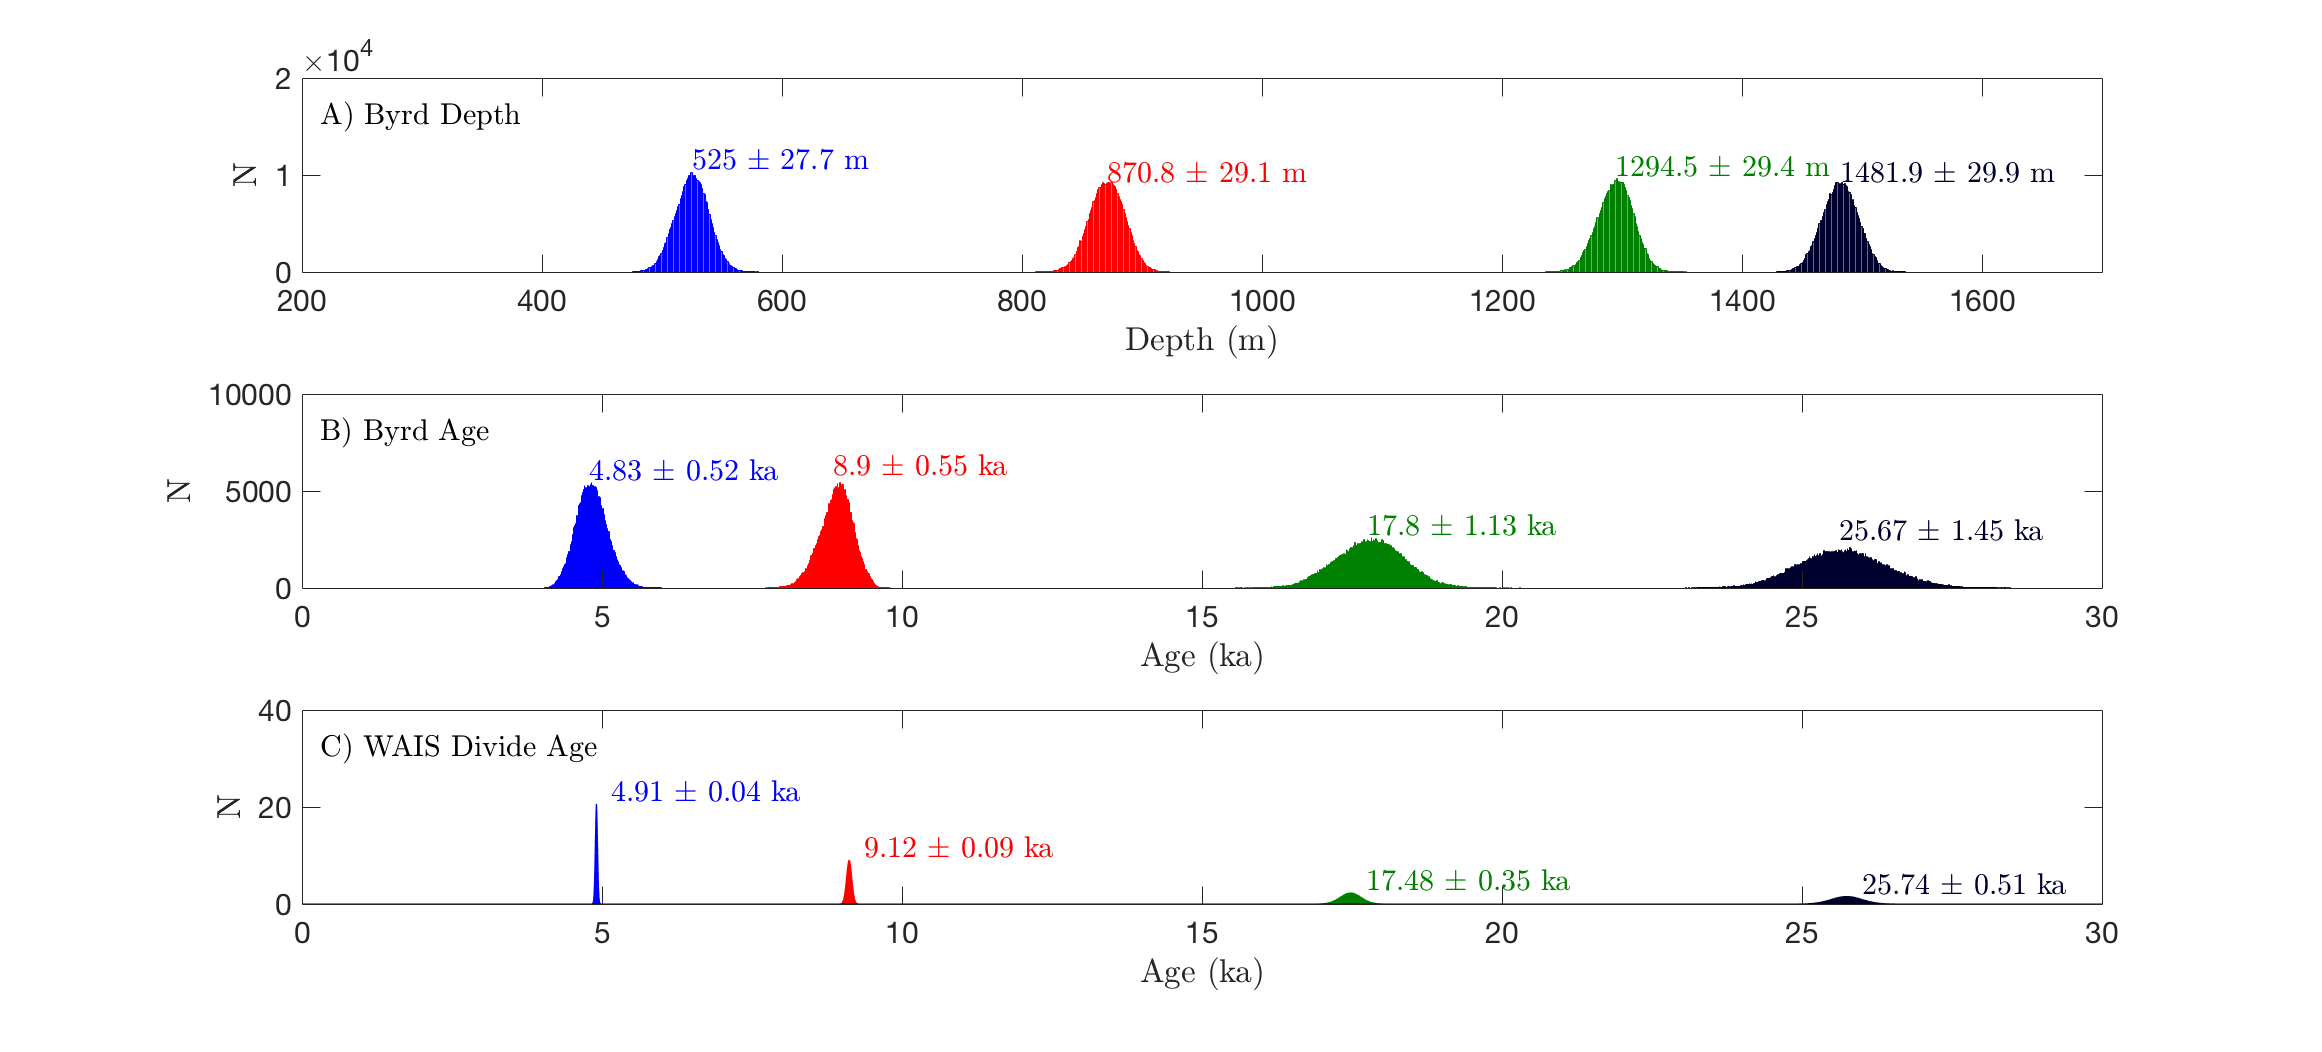
\includegraphics[scale=0.3]{../analysis/figures/agedepthhisto}
%\captionsetup{width=.9\textwidth}
\caption[]{Depth (top) and age (middle) distributions of 4 radar reflectors at the Byrd ice core and the age distribution of the same 4 reflectors at the WAIS Divide ice core (bottom). The width of the age and depth histograms for the Byrd ice core chronology represent uncertainty estimated by the methods used here. The WAIS Divide ice core distributions are recreated from the WAID Divide ice core chronology \cite{buizert2013} and are used as an independent check on our estimation of the age-depth distribution at the Byrd ice core.}
%\end{center}
\label{fig:layer_histo}
\end{figure*}

\begin{figure*}[h]
%\begin{center}
\centering
\includegraphics[scale=0.3]{../analysis/figures/spaghetti}
%\captionsetup{width=.9\textwidth}
\caption[]{Modeled age-depth relationship with uncertainty compared to measured volcanic chronology from \citet[open circles;][]{hammer97}. The WAIS Divide ice core chronogoly \citep{buizert2013} is shown in green. Blue triangles show the age-depth of 5 reflectors at each of the Byrd and WAIS Divide ice cores; these reflectors are assumed isochronous and so expected to be the same age at either ice core.}
%\end{center}
\label{fig:spaghetti}
\end{figure*}

\section{Discussion}\label{discussion}
	For this study, we employ a simplified ice flow model which does not include the effects of upstream ice flow on the reflector ages and assumes one-dimensional vertical strain and constant horizontal strain rate in the upper part of the ice sheet. Below, the model includes shear layer in which horizontal strain decreases linearly to the bed which is allowed to slide. We do not include a separate term for basal melting, which is likely occurring at this site because liquid water was observed at the bed during drilling. Despite this simplification, our results agree with two independent ice core chronologies.

The four reflectors in this study were chosen as a representative sample of the ice column and for their brightness and continuity. It is possible to use this method to date additional englacial reflectors observed using radar in this area. However, the usefulness of such dates only extend as far as the isochronous reflectors can be traced. This method is less helpful for dating discontinuous reflectors, though it could inform relative ages for reflectors seen coincident with dated reflectors but which can be traced only over short distances. 

All such dating efforts should agree to within uncertainty at multiple ice core locations as in \citet{cavitte2016}. We see agreement within 2$\sigma$ between our estimated reflector ages at the Byrd ice core and those observed at the WAIS Divide ice core, though the mean of the latter estimates tend younger than those at the Byrd ice core site. It is unclear why this is the case, though it may be attributable to additional missing uncertainties in drilling of the Byrd ice core. Through use of local density measurements at the WAIS Divide ice core, we exclude differences in firn thickness to account for this discrepancy. However, as an early deep-drilling effort, less sophisticated technology used at the Byrd ice core may have led to more deviations in the drilling direction than reported, for example. Deviations from vertical may lead to a longer core sample than the true ice thickness and may skew the reported volcanic chronology (as measured from the ice core) to be older than it really is. 

Our method is sensitive to the possibility that uncertainty in the estimate of different parameters might be correlated. This is consistent with expectations that parameter values will covary with depth. Because there is not independence between parameters, we must make an assumption about the effective number of degrees of freedom for the ice flow parameters in the problem.  For our age likelihood and estimation of $S$, we assume $k_e$ = 50\% of the number of volcanic data points and do not expect this to change the mean estimates of reflector age and depth, as shown in the Supplemental Information. However, the choice of $k_e$ does have an influence on the uncertainty as indicated in Equation~\ref{eqn:S}.\\





	
\section{Conclusion}\label{conclusion}
	

We derive ages for isochronous radar reflectors observed near Byrd ice core which includes estimates of uncertainty in ice flow parameters and ice properties in the region of Marie Byrd Land, West Antarctica, for which additional observations from radar surveys are just becoming available. Such radar observations reveal englacial stratigraphy indicative of past ice flow, but require dating to put constraints on interpretations of ice dynamics. The Byrd ice core location connects the WAIS divide to the ice streams of the Siple Coast and the Marie Byrd Land icecap, but its chronology has lacked robust estimates of uncertainty until now. 

In addition to estimating uncertainty in the chronology for the full ice column, we estimate the age and depth of four radar reflectors. Our estimates of the reflector age-depth are confirmed by independent comparison to the same reflectors dated using the WAIS Divide ice core chronology \citep{buizert2015}. 

In the process of updating the ice chronology near the Byrd ice core, we also compute self-consistent estimates (with uncertainty) of local ice characteristics, such as the accumulation rate as a function of depth, the firn correction, and the velocity of EM waves in ice. Our method also samples uncertainty in estimates of depth from radar observations. These parameter estimates can be used to inform ice sheet modeling efforts in this area and for other studies of paleo ice flow through the Last Glacial Maximum. 

Our results indicate the oldest continuous radar reflector dateable using existing ice cores and radar surveys in West Antarctica is located at $\sim$70\% ice depth at the Byrd ice core site and dates to $\sim$ 26 ka. The same reflector is observed at $~\sim$80\% ice depth in the WAIS Divide ice core. While the Byrd ice core has been isotopically dated to as old as $\sim$ 94 ka \citep{blunier2001}, continuous radar reflectors do not extend deep enough in this region to leverage the ice core to date older aspects of the ice geometry in the central WAIS.








%%% End of body of article:

%%%%%%%%%%%%%%%%%%%%%%%%%%%%%%%%
%% Optional Appendix goes here
%
% \appendix resets counters and redefines section heads
% but doesn't print anything.
% After typing  \appendix
%
% \section{Here Is Appendix Title}
% will show
% Appendix A: Here Is Appendix Title
%

%\appendix
%	\renewcommand{\thepage}{S\arabic{page}}  
\renewcommand{\thesection}{S\arabic{section}}   
\renewcommand{\thetable}{S\arabic{table}}   
\renewcommand{\thefigure}{S\arabic{figure}}
\setcounter{figure}{0}

\section{Metropolis Evaluation}
\counterwithin{figure}{section} %reset figure numbering

The metropolis algorithm was evaluated for 450,000 iterations, with the first 10,000 discarded as ``burnin" iterations, during which the model was experiencing transient behavior. Such a large number of iterations allows for convergence of all parameters to their best solutions. Our method is based on a markov chain, such that the proposed parameter values for each iteration depend on the values from the last accepted iteration according to:
\begin{equation}\label{eqn:proposal}
\begin{split}
delta&=Range(Prior) \\
Proposal_i&=Accepted_{i-1} + dp \cdot (0.5-rand) \cdot delta; 
\end{split}\tag{S1}
\end{equation}
where $delta$ is the range allowed by the uniform prior for each parameter and $rand$ is a random number between 0 and 1. $Proposal_i$ is the value of a parameter for iteration $i$ and $Accepted_{i-1}$ is the previous value of that parameter accepted by the algorithm. To more efficiently explore parameter space, proposed parameters were selected with step sizes $dp_{Age}$ = 0.1 and $dp_{TWTT}$ = 0.1 for those parameters associated with each likelihood in Equation~\ref{eqn:bigproblem}.

The evaluation of the two likelihood functions (i.e. ``cost") are independently accepted according to each function's metropolis probability during each iteration. The accepted solutions for each cost, depth, and age are shown in Figure~\ref{fig:cost}. As seen in the figure, these cost values show little trend aside from occasional positive departures from the mean as the model explores parameter space. 

\begin{figure*}[ht]
%\begin{center}
\centering
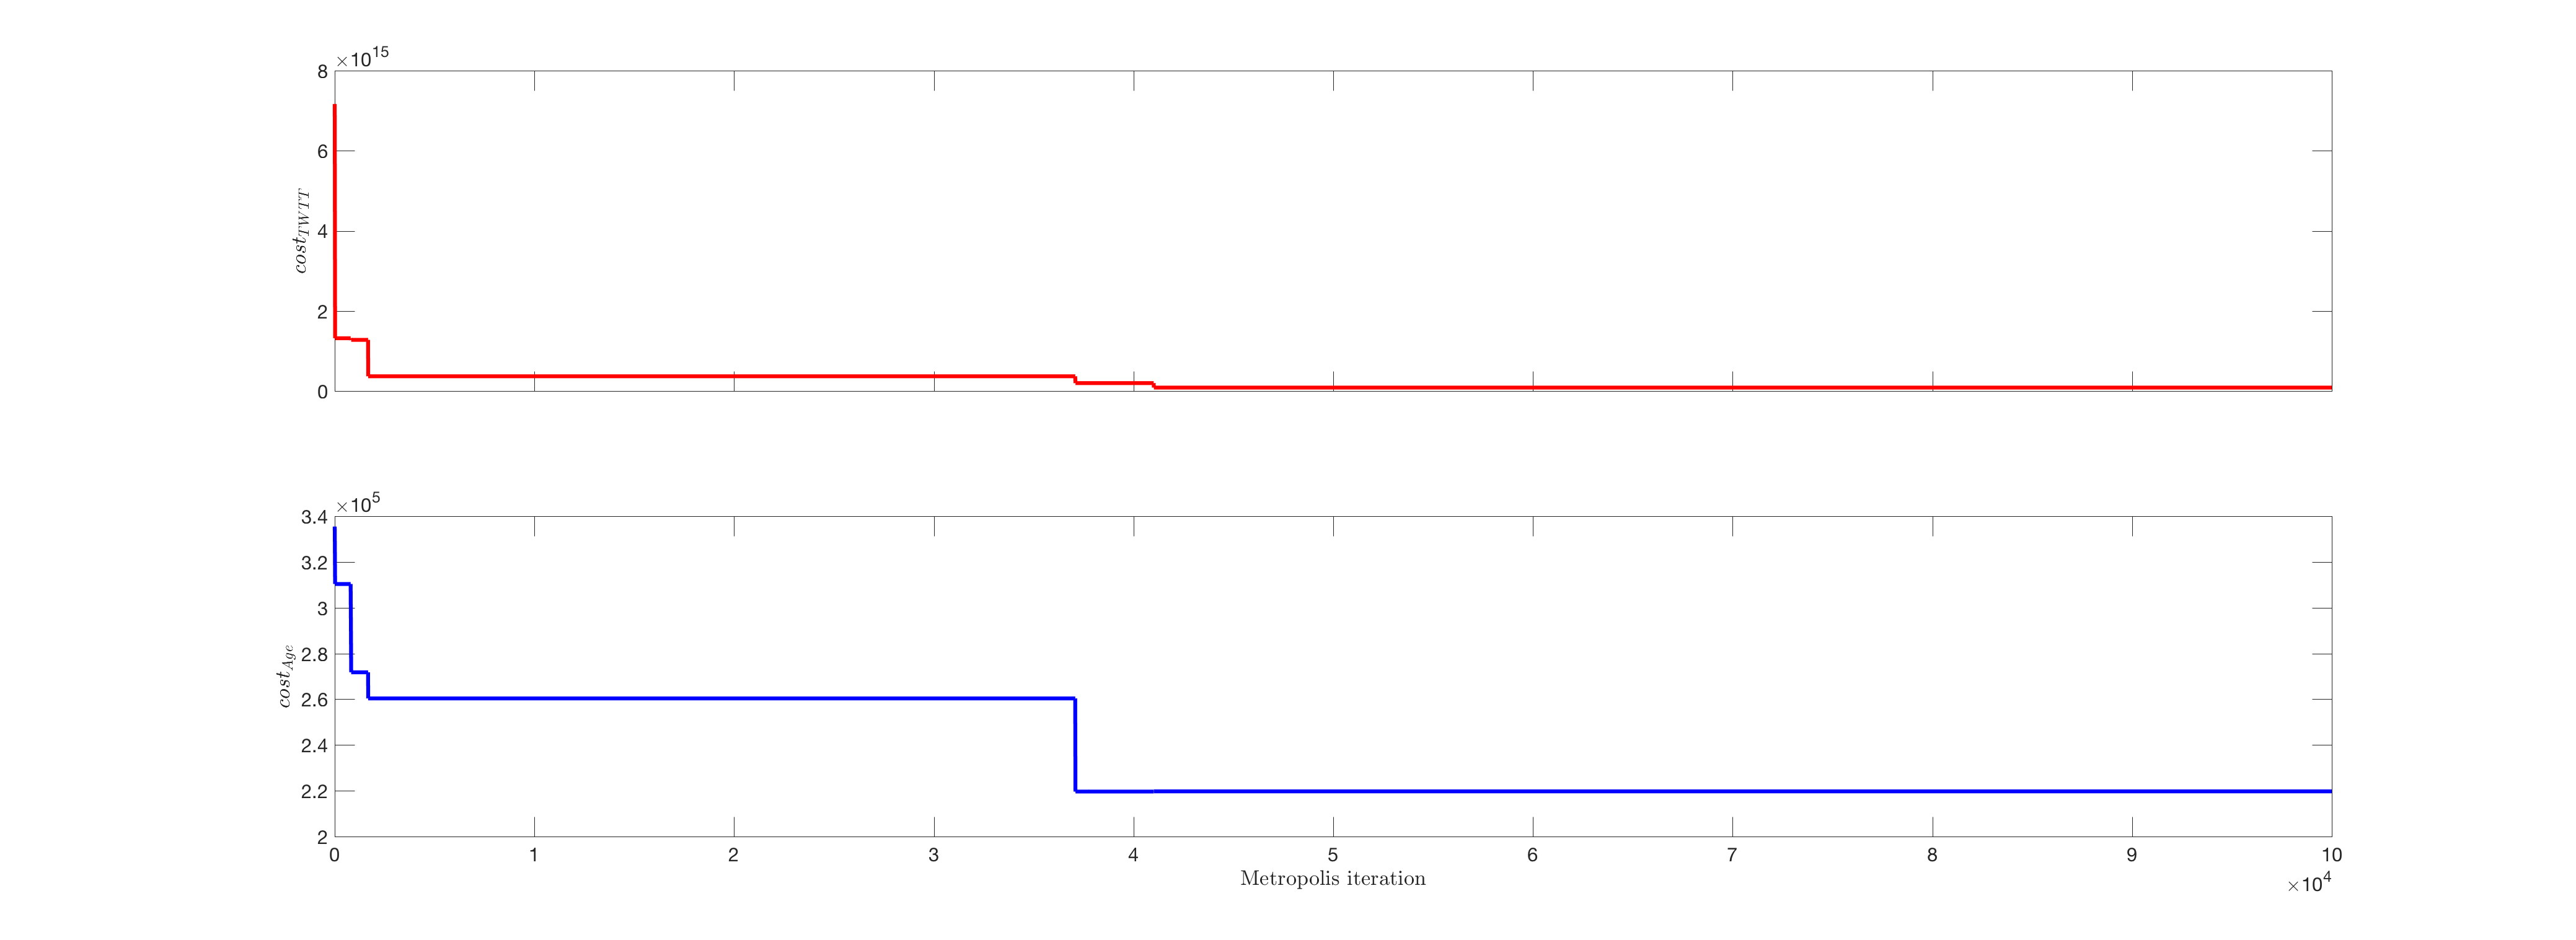
\includegraphics[scale=0.4]{../analysis/figures/cost}
%\captionsetup{width=.9\textwidth}
\caption[]{Cost of the age and depth likelihood functions at each accepted iteration.}
%\end{center}
\label{fig:cost}
\end{figure*}





\section{Regularization}\label{sec:regularization}
\counterwithin{figure}{section} %reset figure numbering

Sampling accumulation rate parameters along the depth profile is inefficient and problematic because many proposed solutions are unrealistically variable. We expect the mean accumulation rate over time (and therefore depth) changes slowly and continuously. To improve our accumulation rate solutions, we regularize the likelihood of reflector age. A regularization parameter is added to the age cost term which punishes proposed accumulation rate profiles which are highly variable relative to a solution computed with no regularization and smoothed over a moving 600-m depth window. This window size is chosen because it is the smallest interval over which the data can be smoothed given the 200-m bin size of the accumulation rate parameters. 

The regularization term, $r$ is the ratio of the variance of a proposed set of accumulation rates to the variance of the smoothed, non-regularized accumulation rate profile. Values of the regularization term for accepted parameter solutions are shown in Figure~\ref{fig:reg}. The regularization is weighted as $r^6$ when included in the calculation of the age cost (Equation~\ref{eqn:loglikeage}) to sufficiently reduce variability in the accumulation rate profile. 


\begin{figure*}[ht]
%\begin{center}
\centering
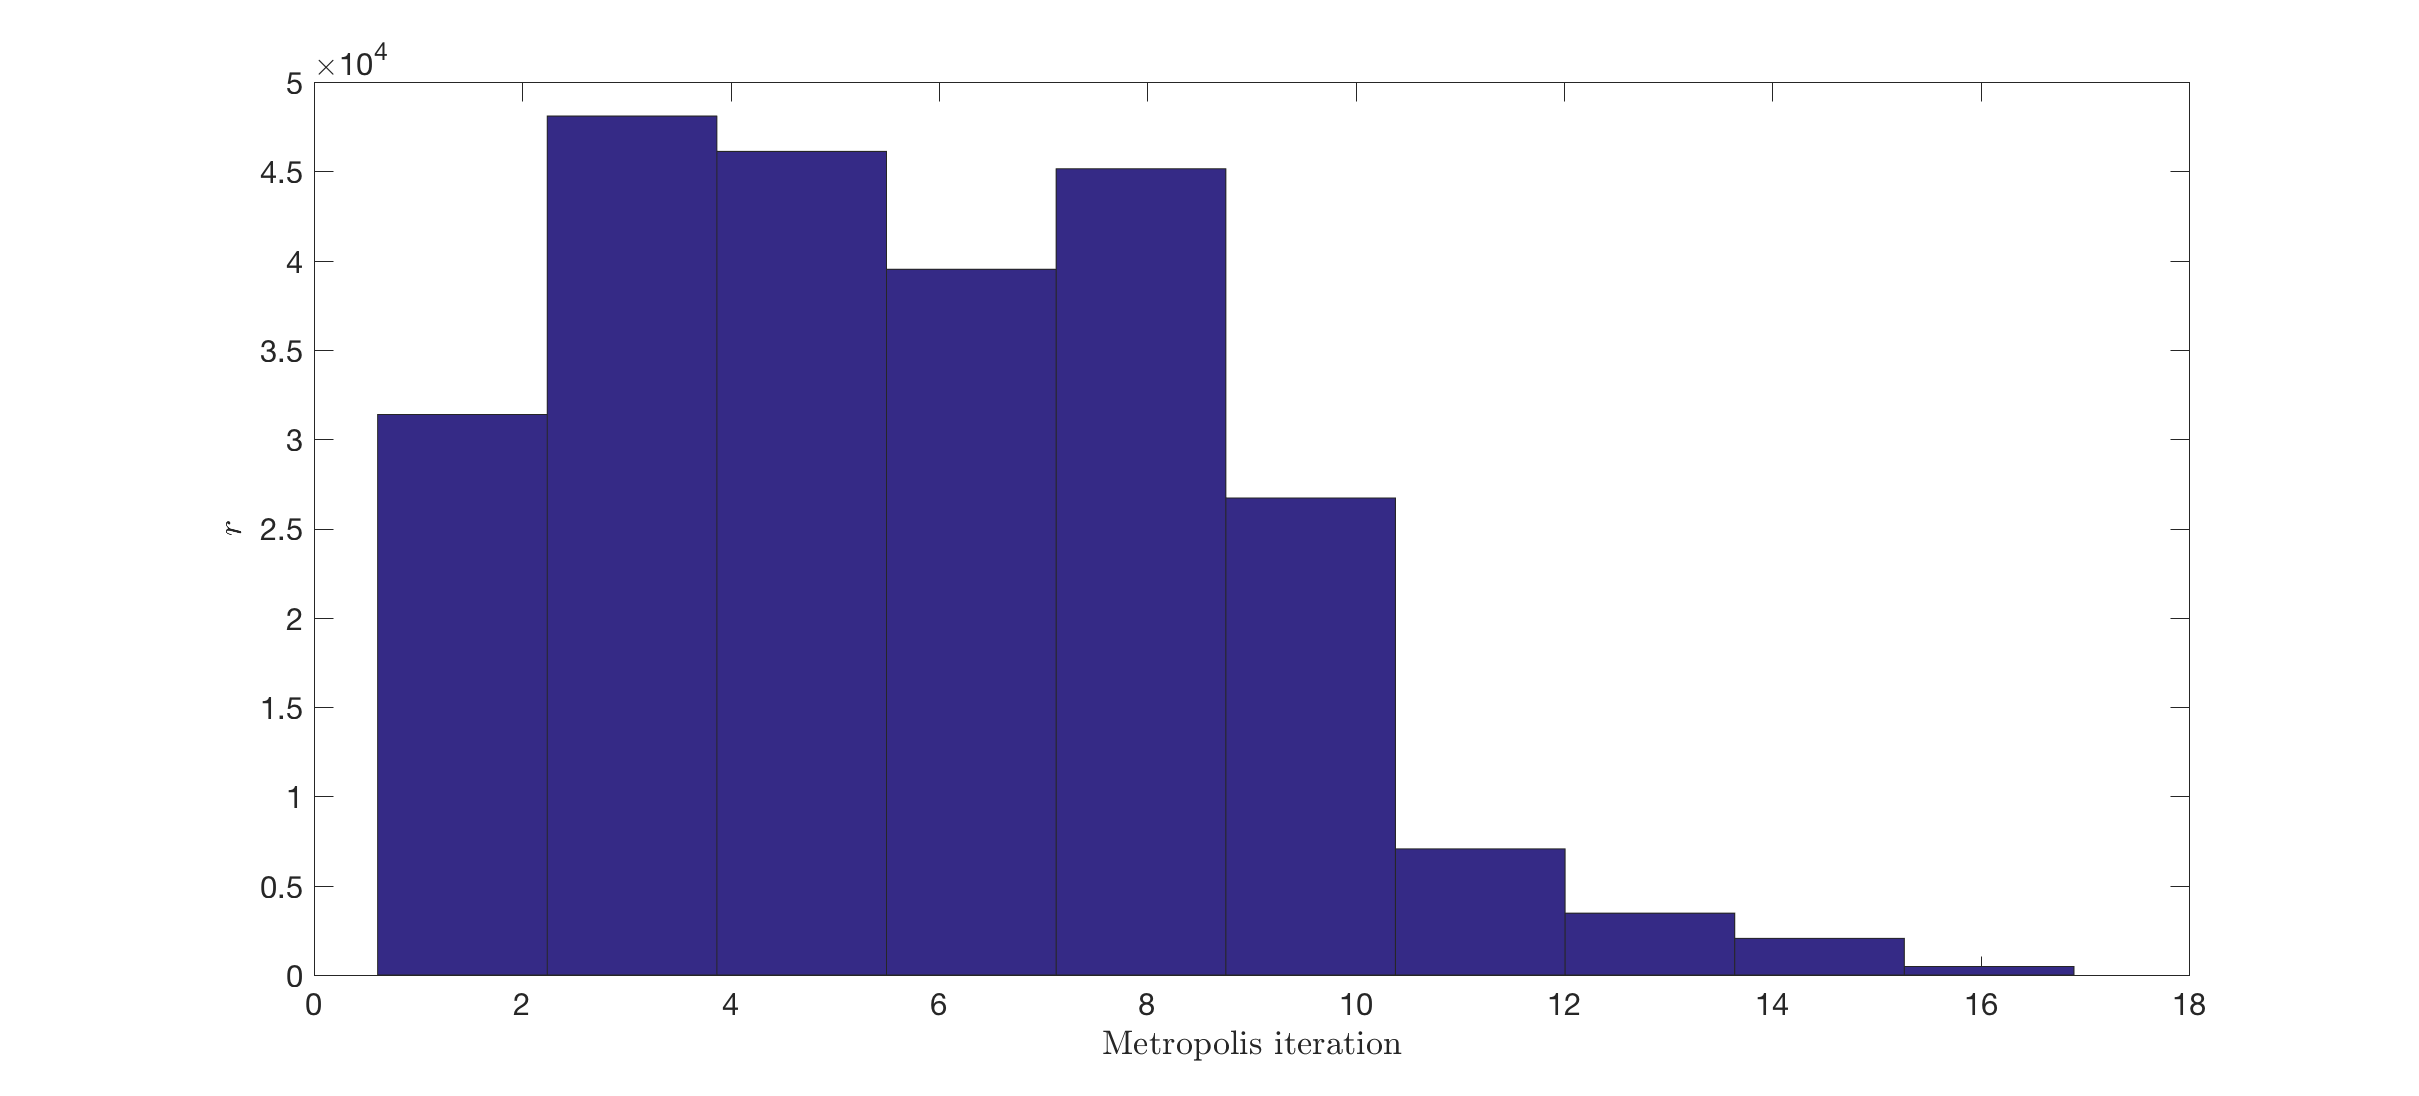
\includegraphics[scale=0.4]{../analysis/figures/regularization}
%\captionsetup{width=.9\textwidth}
\caption[]{Values of the regularization parameter at each accepted metropolis iteration.}
%\end{center}
\label{fig:reg}
\end{figure*}








\section{Estimating TWTT uncertainty}\label{sec:sigmatwtt}
\counterwithin{figure}{section} %reset figure numbering
To estimate $\sigma_{TWTT}$ in Equation~\ref{eqn:loglikeage}, we assume a perfect model then perturb it with errors consistent what we expect to find in the data. We assume the depth errors can be described by a gaussian distribution which results in the following relationship between the cost, degrees of freedom, and $\sigma_{TWTT}$ \citep{jackson&huerta2016}.


\begin{equation}
\frac{1}{\sigma_{TWTT}}= \frac{\sqrt{k_e/2}}{\sigma_{{E_m}^*}}\tag{S2}
\end{equation}
Here $k_e$ is the effective number of degrees of freedom and ${E_m}^*$ represents the perfect model of TWTT which is perturbed with errors consistent with what we expect to find in the radar observations. For simplicity, we assume $k_e$ is the same as the number of reflectors for which we invert.

This method makes use of the ``perfect model":
\begin{equation}
cost^*_{TWTT} = \frac{\sum_{j = z}[TWTT_m(z) - \overline{TWTT_m}(z)]^2}{2}
\end{equation}


% \section{Byrd ice core volcanic chronology}\label{sec:volcanic}

% Table of those points from the 50ka record used (i.e. ones with unique depths at 1-m model resolution)





\section{Degrees of freedom and parameter correlation}\label{sec:ke}
\counterwithin{figure}{section} %reset figure numbering

As we invert for model parameter values, we anticipate the data points used to constrain our likelihood functions -- sourced from radar observations and a Byrd ice core volcanic chronology -- are not independent of one another. As a result, we expect the number of degrees of freedom to be less than the number of data points available. While we do not know the number of effective degrees of freedom, $k_e$, we explore the sensitivity of our results to our choice of $k_e$ (Figure~\ref{fig:ke}). We find that our choice does not significantly impact the mean estimates of age or depth for our radar reflectors. In lieu of more information about the degrees of freedom, we choose to assume $k_e = \frac{N_{data}}{2} = 30.5$ because convergence on the accumulation rates are strong and the rate at which the algorithm finds solutions is reasonable. 

\begin{figure*}[ht]
\begin{center}
%\centering
\makebox[\textwidth][c]{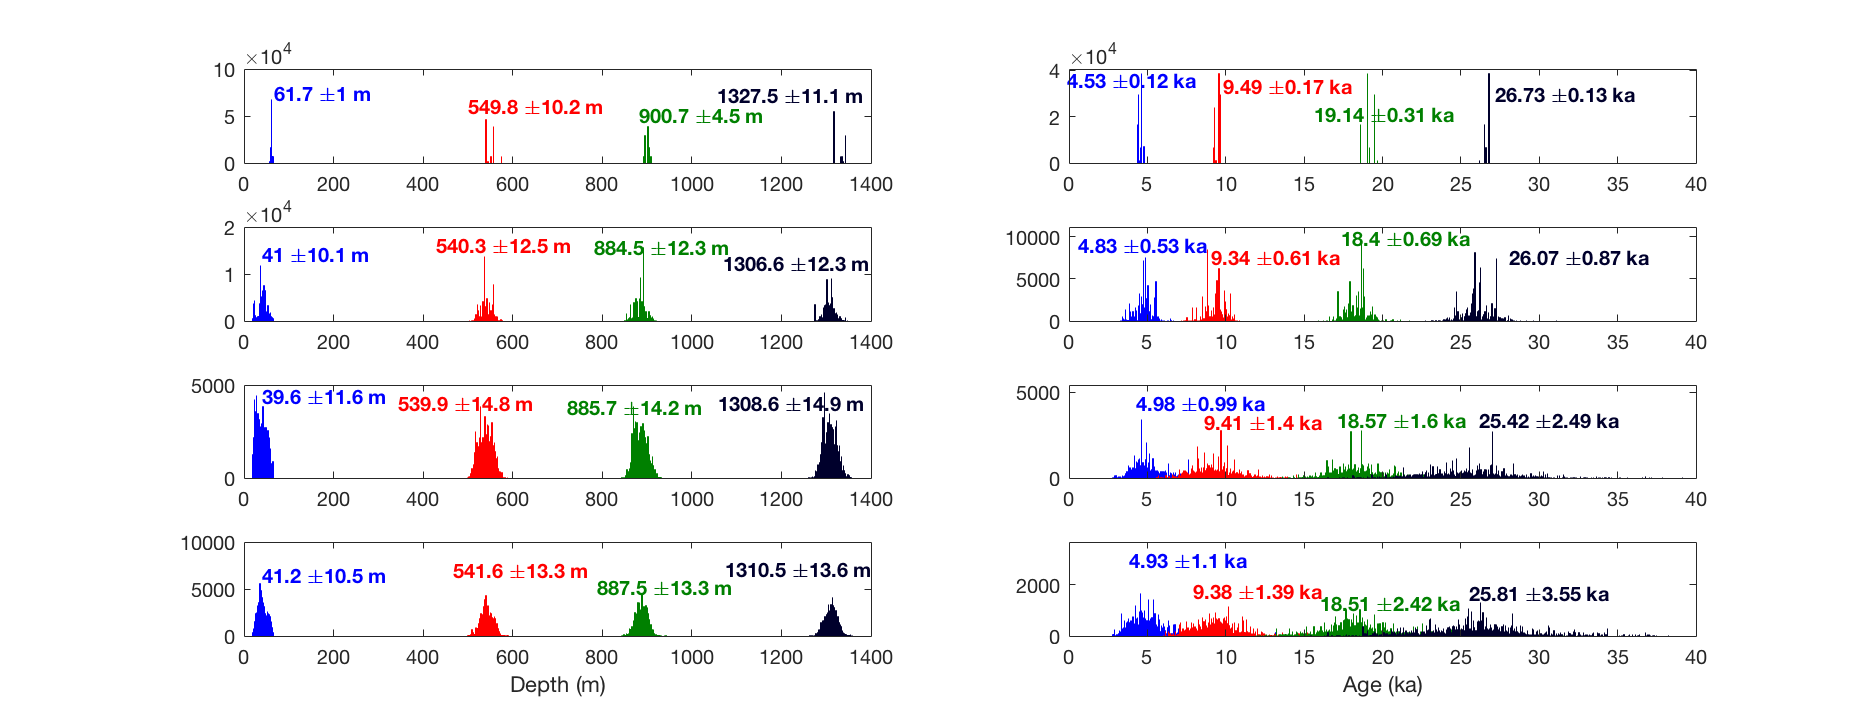
\includegraphics[scale=0.35]{../analysis/figures/keCompare_tweaked}}
%\captionsetup{width=.9\textwidth}
\caption[scale=0.3]{Comparison of results for reflector age and depth assuming a range of $k_e$ values. All agree to within uncertainty.}
\end{center}
\label{fig:ke}
\end{figure*}

Figure~\ref{fig:flowparamconvergence} shows the results of inverting for several model parameters in this problem, including flow parameters such as $q$ as well as ice property parameters such as $v_{ice}$. The results show the parameters are not correlated with one another and do seem to convergence to most-likely solutions.

\begin{figure*}[ht]
%\begin{center}
\centering
\makebox[\textwidth][c]{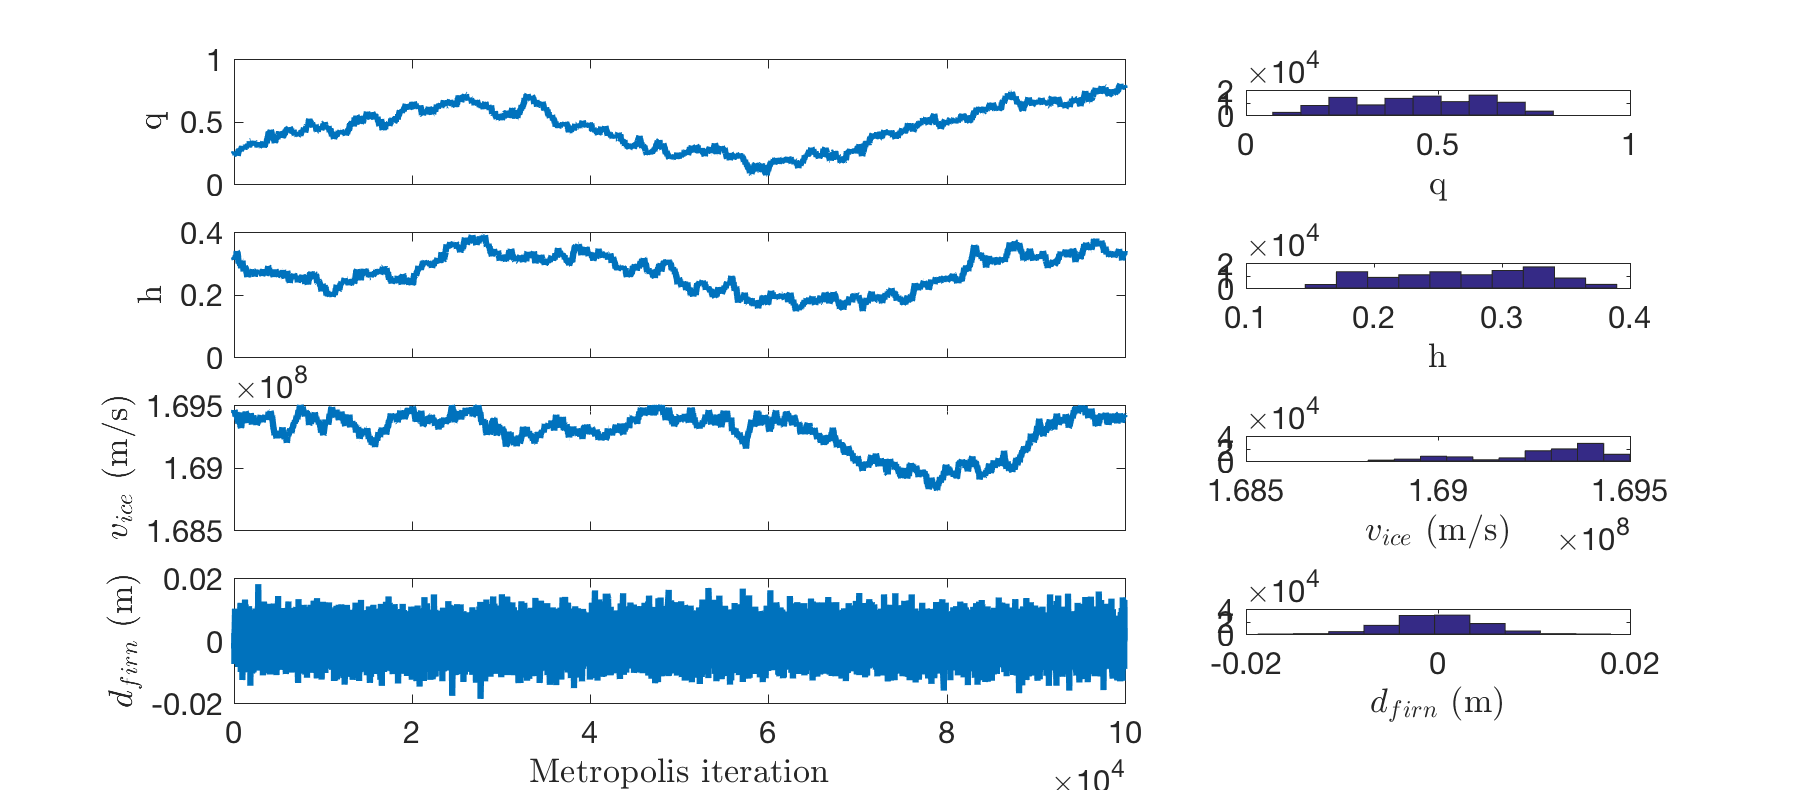
\includegraphics[scale=0.4]{../analysis/figures/convergence1}}
%\captionsetup{width=.9\textwidth}
\caption[]{Left: Flow parameter values at each accepted Metropolis iteration for parameters $q$ (top), $h$, $v_{ice}$, and $d_{firn}$ (bottom). The parameter values do not appear correlated Right: Histograms of the parameter values shown in the left column. Histograms show the parameter values converging.}
%\end{center}
\label{fig:flowparamconvergence}
\end{figure*}

Accumulation rate is divided into 10 parameters, each covering a depth bin of $\sim$200 m. This allows for variation in the accumulation rate over time, as expected. The resulting accumulation rate profiles are shown in Figure~\ref{fig:accumdepth}. As discussed elsewhere in the Supplemental Information, these profiles have been regularized to preferentially select those which do not exhibit unrealistic variability. In Figure~\ref{fig:accumdepth}, they have been additionally sorted by cost to demonstrate the relative quality of the accepted solutions.

\begin{figure*}[ht]
%\begin{center}
\centering
\makebox[\textwidth][c]{\includegraphics[scale=0.4]{../analysis/figures/accumdepthSorted}}
%\captionsetup{width=.9\textwidth}
\caption[]{Accumulation rate as a function of ice depth colored by cost value for the estimated parameter values. (Accumulation rate series associated with lower cost are expected to be solutions.) Accumulation rate is estimated in 10 depth bins at $\sim$200 m depth intervals. Transitions between these intervals have been smoothed in this figure for each of viewing.}
%\end{center}
\label{fig:accumdepth}
\end{figure*}

To further explore the accumulation rate solutions, we look at the accepted parameter values and their convergence over all iterations. As seen in the right side of Figure~\ref{fig:accumconvergence}, the accumulation rate solutions do not converge as readily as other parameters, leaving wider distributions exhibiting more uncertainty in our estimates of accumulation rate. This may mean that our priors play an important role in estimating the value of accumulation rate and therefore the result could be improved with a more informative prior. This is particularly true at the bottom of the ice column, where neither volcanic chronology data nor radar data is available to constrain the accumulation rate.

We see correlation between some accumulation rate parameters (left side of Figure~\ref{fig:accumconvergence}). This may indicate we could have combined these accumulation rate depth bins. Figure~\ref{fig:accumCorrelation} shows a correlation matrix between pairs of accumulation rate parameters. Along the diagonal are histograms of each accumulation rate parameter. Pairs of accumulation rate parameters to not tend to be very correlated and only one pair of accumulation rate parameters has $R^2 > 0.5$. In general, $R^2$ values are highest between accumulation rates in the lower part of the ice column, where parameter values are more difficult to constrain due to a lack of data and flatter age-depth profile.


\begin{figure*}[ht]
%\begin{center}
\centering
\makebox[\textwidth][c]{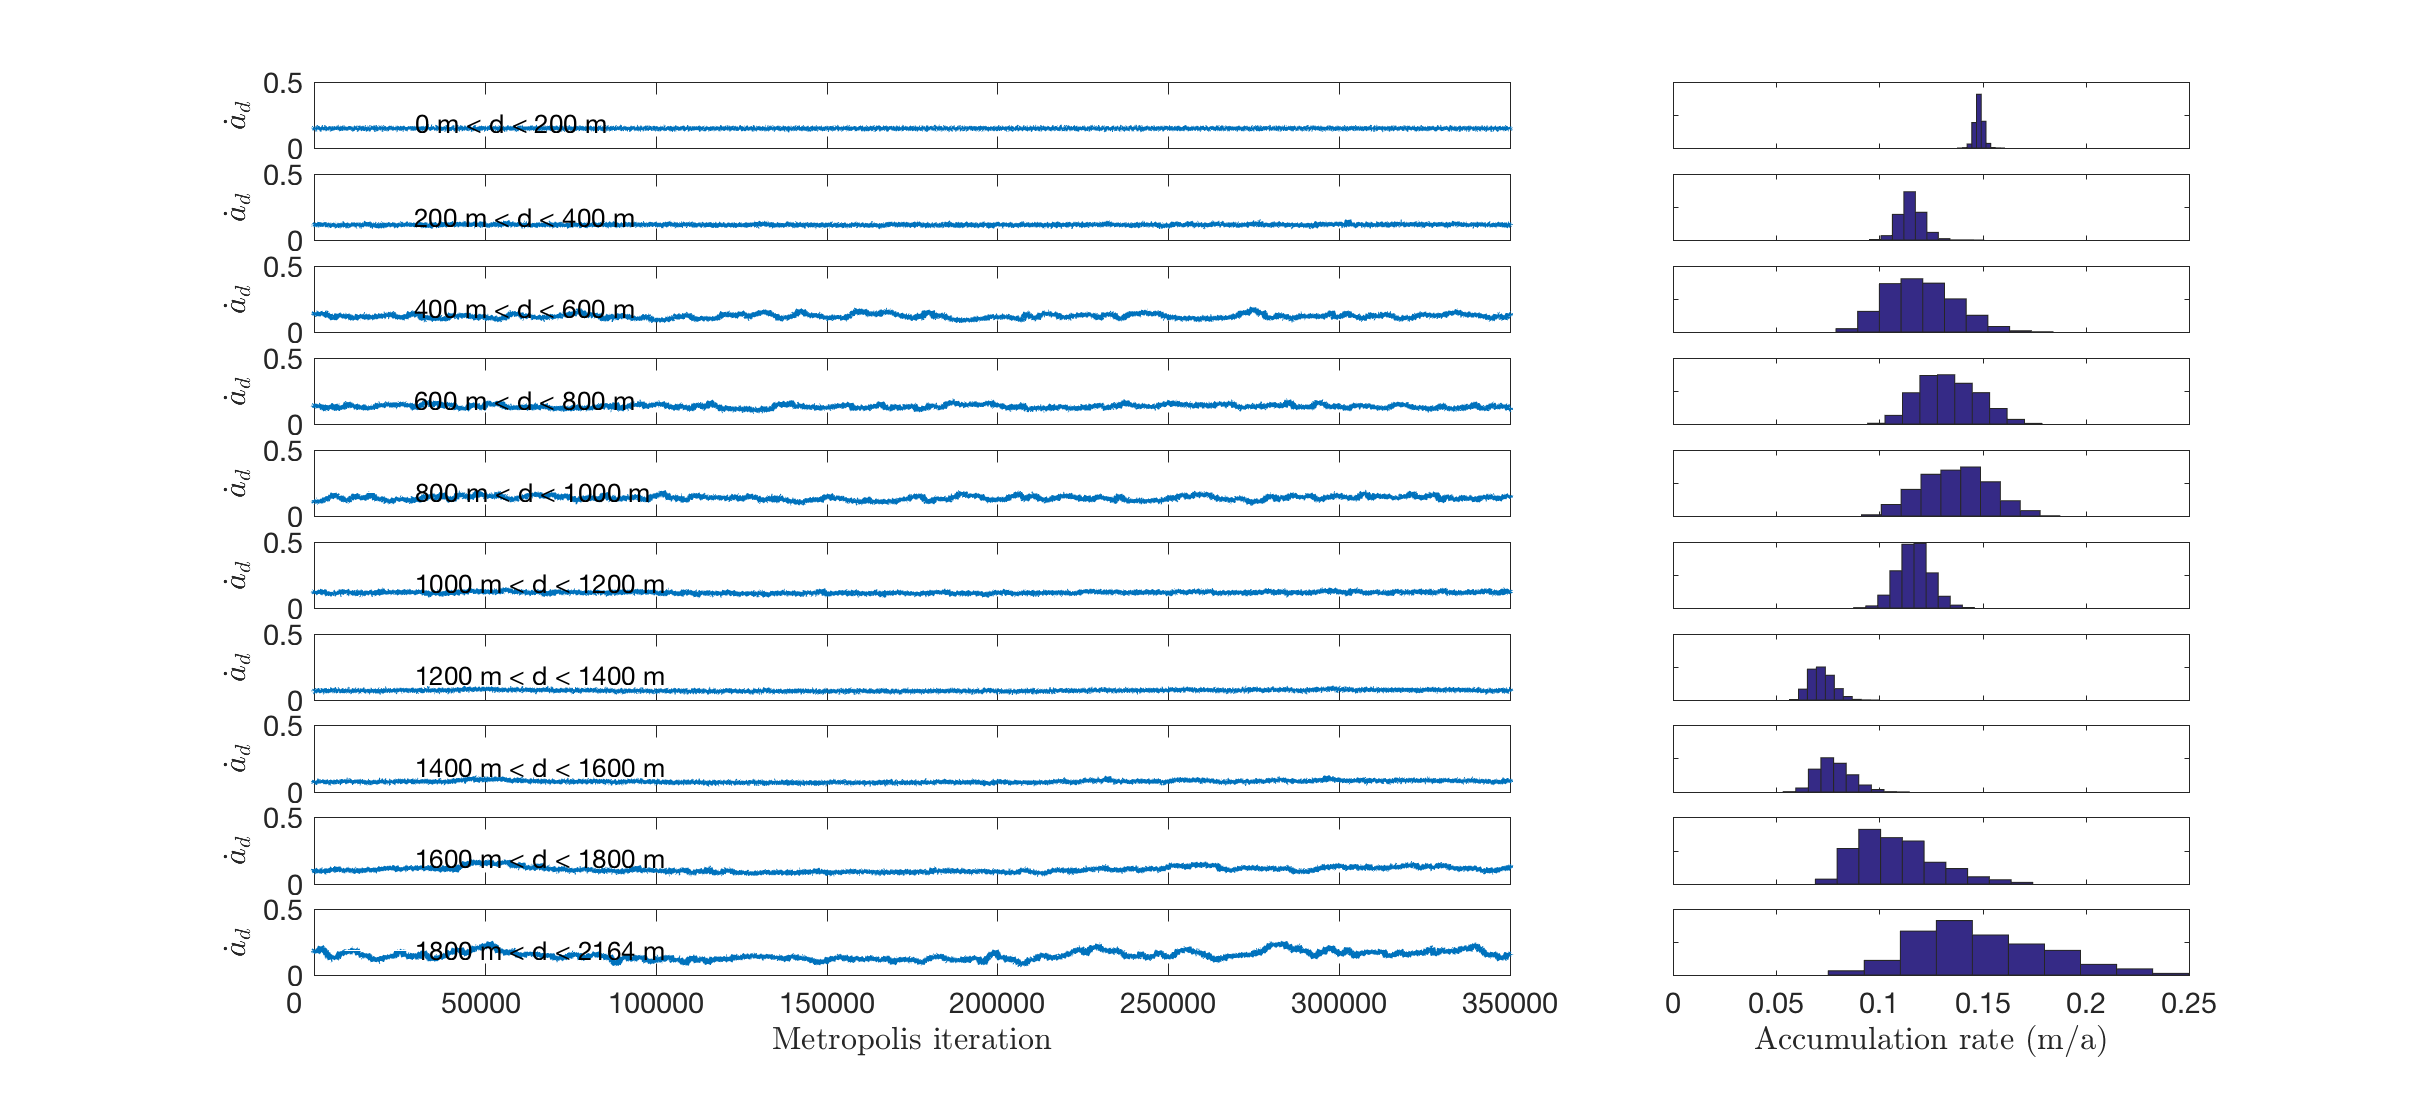
\includegraphics[scale=0.4]{../analysis/figures/convergence2}}
%\captionsetup{width=.9\textwidth}
\caption[]{Left: Values of each accumulate rate parameter (in each of 10 depth bins, shallowest at top). Right: Histograms of the parameter values at left. Certain depth bins appear to be correlated and the histograms of values are wider, indicating the accumulation rate parameters are slower to converge and more uncertain.}
%\end{center}
\label{fig:accumconvergence}
\end{figure*}

\begin{figure*}[ht]
%\begin{center}
\centering
\makebox[\textwidth][c]{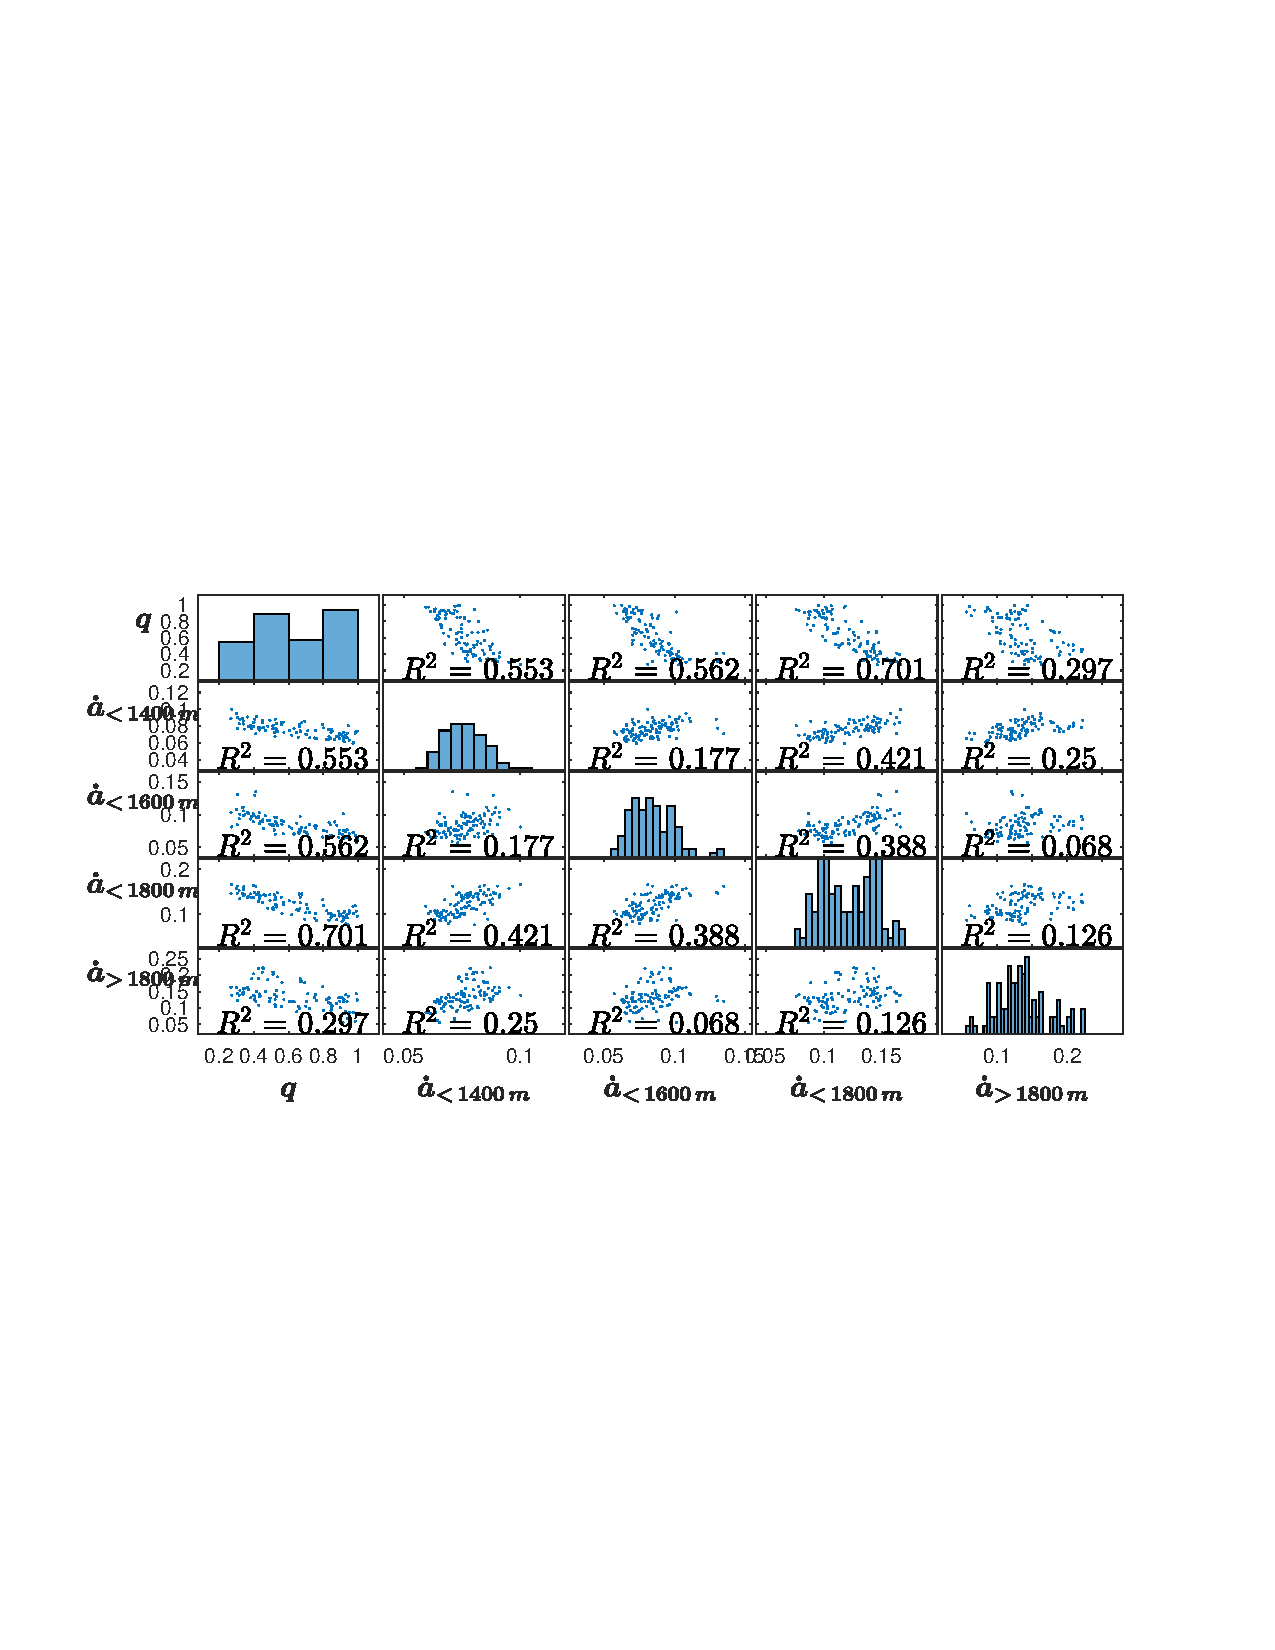
\includegraphics[scale=0.4]{../analysis/figures/accumCorrelation}}
%\captionsetup{width=.9\textwidth}
\caption[]{Correlation of each accumulation rate parameter with every other accumulation rate parameter. Histograms of each accumulation rate are shown along the diagonal. Pairs of parameters with $R^2 > 0.5$ have their correlation coefficients shown in red.}
%\end{center}
\label{fig:accumCorrelation}
\end{figure*}


% Convergence of the reflector depths is shown in Figure~\ref{fig:depthconvergence}.


% \begin{figure*}[ht]
% %\begin{center}
% \centering
% \makebox[\textwidth][c]{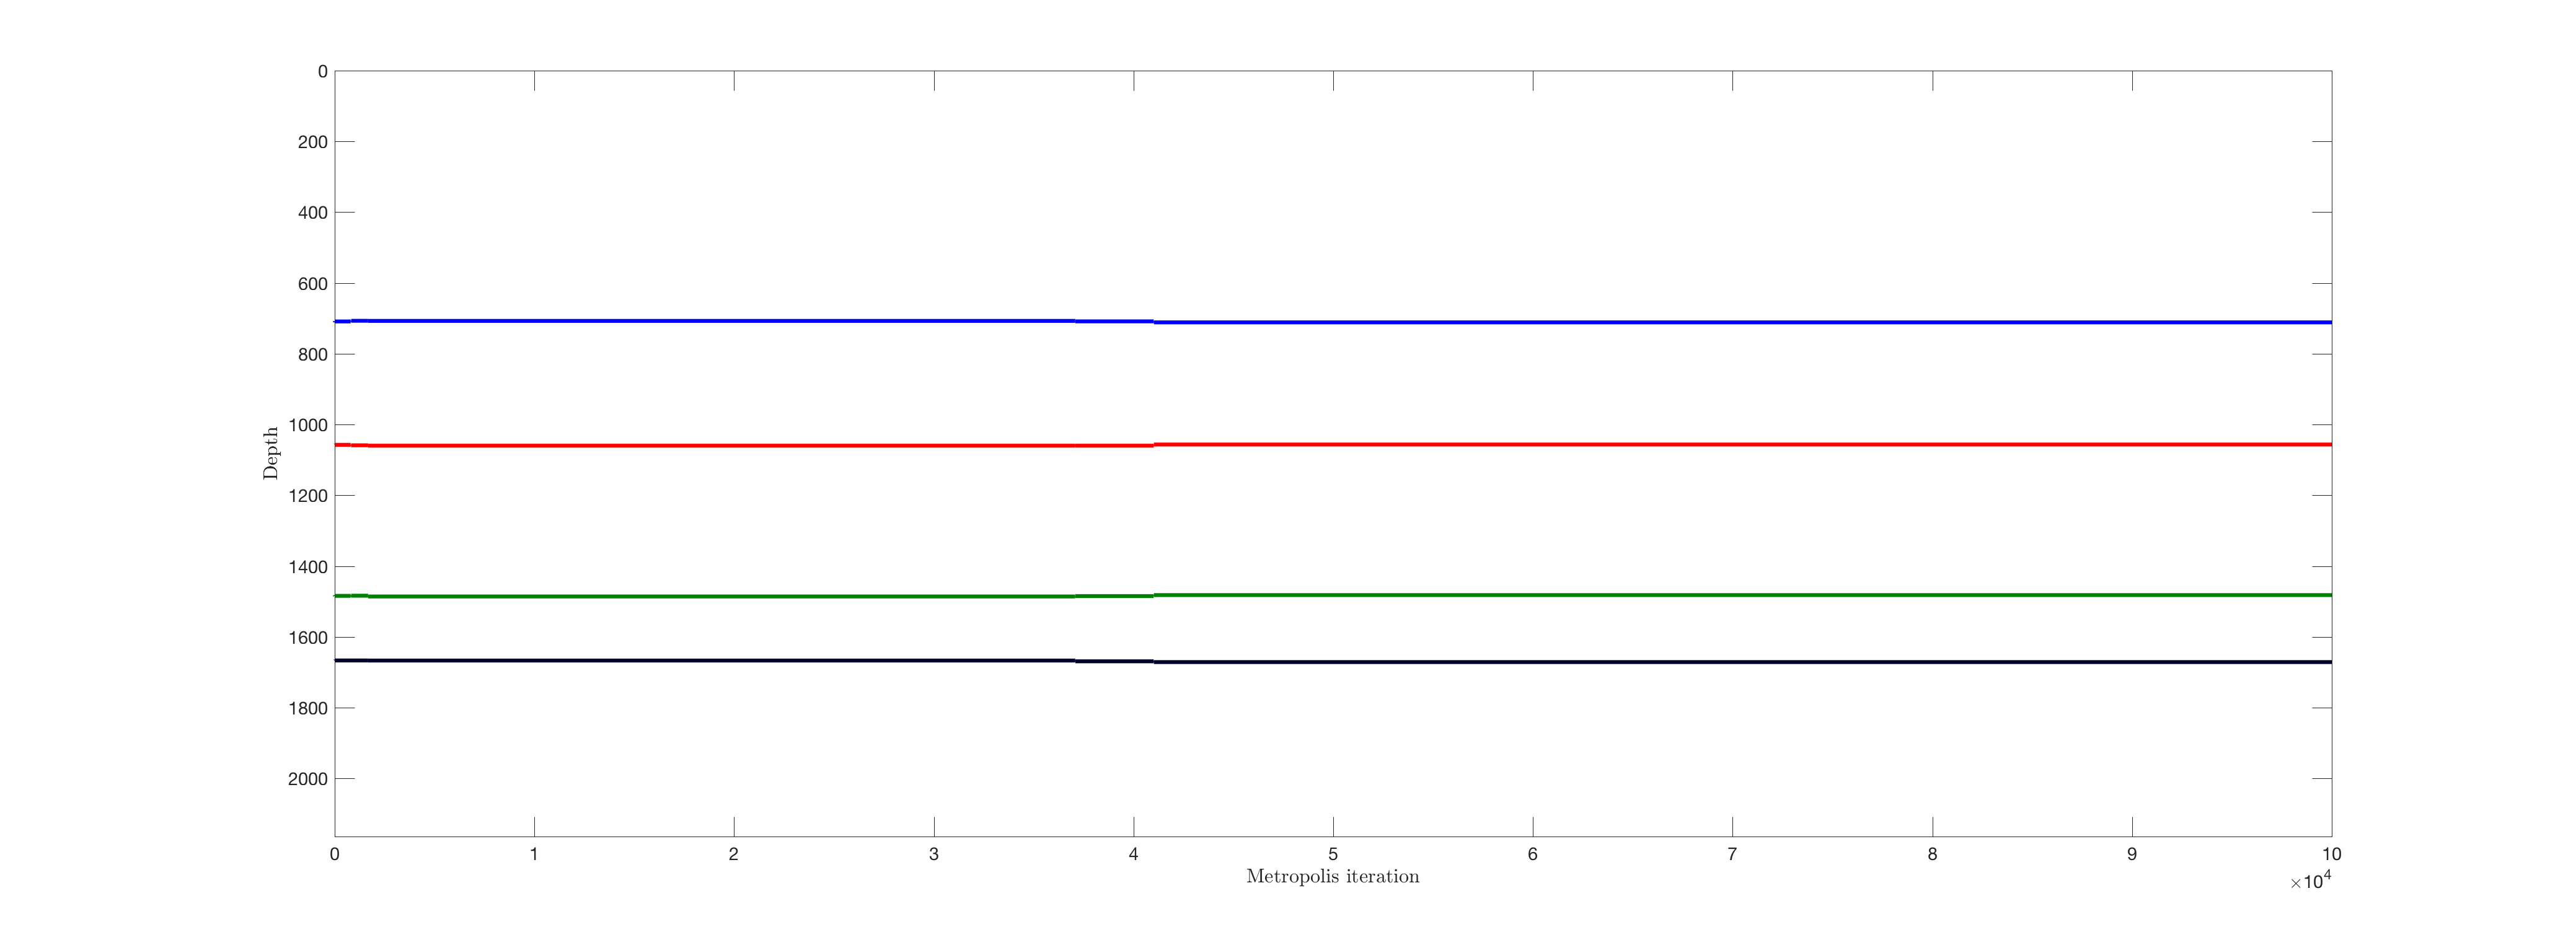
\includegraphics[scale=0.4]{../analysis/figures/convergence3}}
% %\captionsetup{width=.9\textwidth}
% \caption[]{Reflector depth values at each accepted metropolis iteration.}
% %\end{center}
% \label{fig:depthconvergence}
% \end{figure*}



% \section{Firn Correction}

% \begin{figure*}[h]
% %\begin{center}
% \centering
% 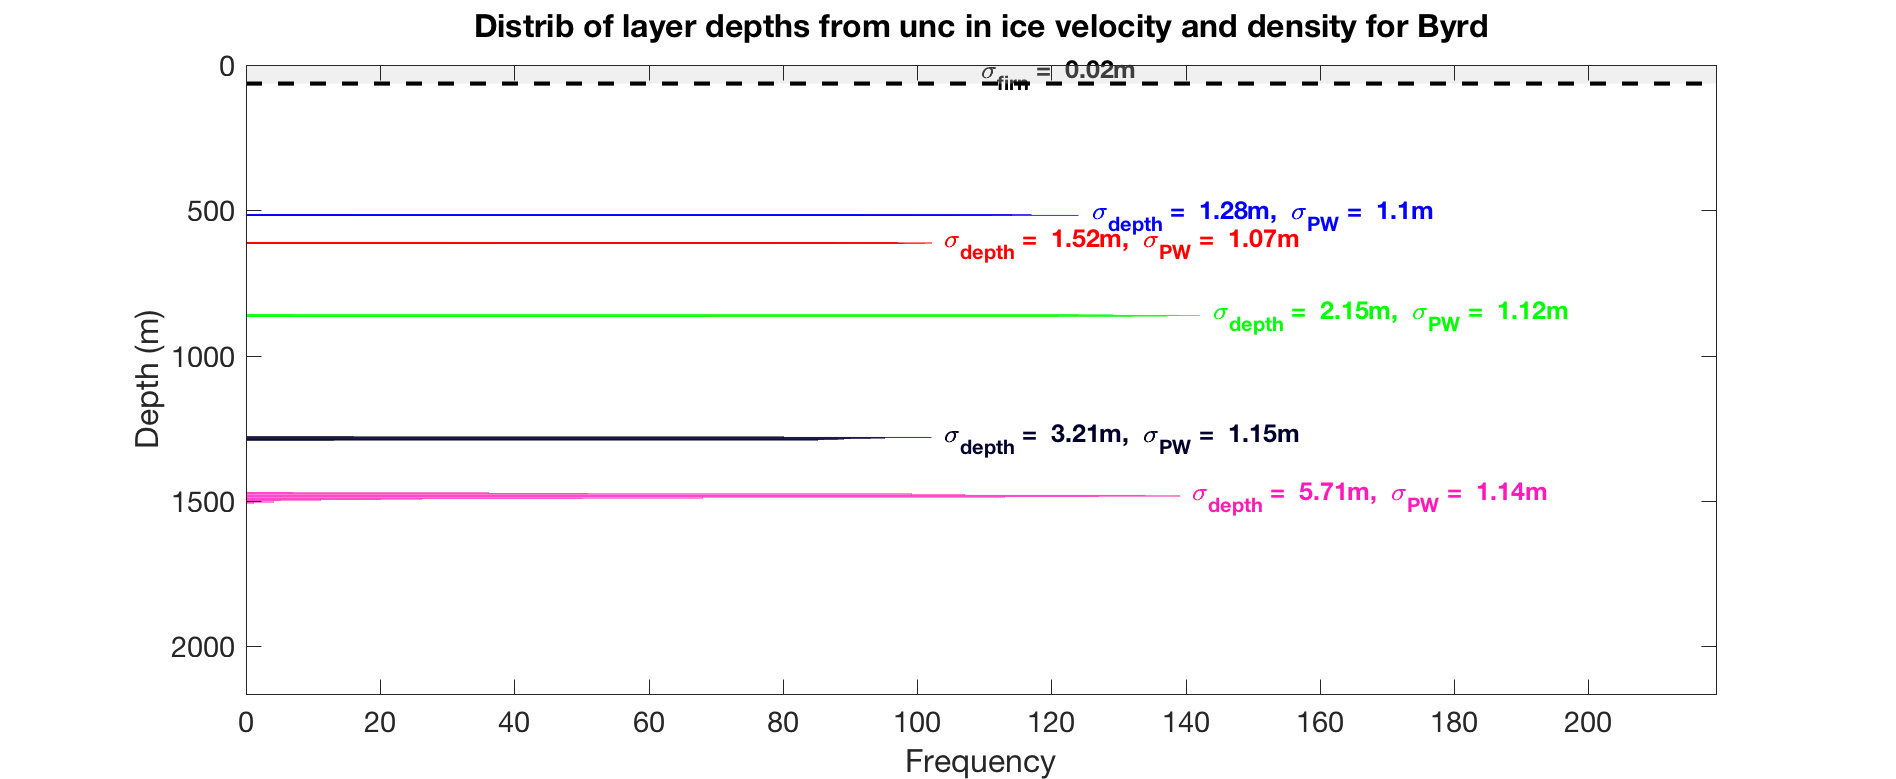
\includegraphics[scale=0.5]{figures/firncorrection}
% %\captionsetup{width=.9\textwidth}
% \caption[]{}
% %\end{center}
% \label{fig:firncorrection}
% \end{figure*}










%%%%%%%%%%%%%%%%%%%%%%%%%%%%%%%%%%%%%%%%%%%%%%%%%%%%%%%%%%%%%%%%
%
% Optional Glossary or Notation section, goes here
%
%%%%%%%%%%%%%%
% Glossary is only allowed in Reviews of Geophysics
% \section*{Glossary}
% \paragraph{Term}
% Term Definition here
%
%%%%%%%%%%%%%%
% Notation -- End each entry with a period.
% \begin{notation}
% Term & definition.\\
% Second term & second definition.\\
% \end{notation}
%%%%%%%%%%%%%%%%%%%%%%%%%%%%%%%%%%%%%%%%%%%%%%%%%%%%%%%%%%%%%%%%
%
%  ACKNOWLEDGMENTS

\begin{acknowledgments}
The authors thank UTIG radar interpreters including Robert Stephany, Shubhanga Ballal, Arami Rosales, Rebekah Albach, and Varun Sudunagunta. Funding for this project came from the University of Texas Institute for Geophysics, CDI (NSF Grant \# OPP-0941678), SPICECAP (NSF Grant \#PLR-1443690), GIMBLE (NSF Grant \#PLR-1043761), and The G.  Unger Vetlesen Foundation. 
\end{acknowledgments}

%% ------------------------------------------------------------------------ %%
%%  REFERENCE LIST AND TEXT CITATIONS
%
% Either type in your references using
% \begin{thebibliography}{}
% \bibitem{}
% Text
% \end{thebibliography}
%
% Or,
%
% If you use BiBTeX for your references, please produce your .bbl
% file and copy the contents into your paper here.
%
% Follow these steps:
% 1. Run LaTeX on your LaTeX file.
%
% 2. Run BiBTeX on your LaTeX file.
%
% 3. Open the new .bbl file containing the reference list and
%   copy all the contents into your LaTeX file here.
%
% 4. Comment out the old \bibliographystyle and \bibliography commands.
%
% 5. Run LaTeX on your new file before submitting.
%
% AGU DOES NOT WANT a .bib or a .bbl file. Please copy in the contents of your .bbl file here.

%*************\begin{thebibliography}{}

%\bibitem[{\textit{Kilby}(2008)}]{jskilby}
%Kilby, J. S. (2008), Invention of the integrated circuit, {\it IEEE
%Trans. Electron Devices,} \textit{23}, 648--650.

%\bibitem[{\textit{Kilby et al.}(2008)}]{jskilbye}
%Kilby, J. S., S. Smith, and R. Jones (2008), Invention of the
%integrated circuit, {\it IEEE Trans. Electron Devices,} \textit{23},
%648--650.
\bibliographystyle{agu}
\bibliography{bib}
%***************\end{thebibliography}

%Reference citation examples:

%...as shown by \textit{Kilby} [2008].
%...as shown by {\textit  {Lewin}} [1976], {\textit  {Carson}} [1986], {\textit  {Bartholdy and Billi}} [2002], and {\textit  {Rinaldi}} [2003].
%...has been shown [\textit{Kilby et al.}, 2008].
%...has been shown [{\textit  {Lewin}}, 1976; {\textit  {Carson}}, 1986; {\textit  {Bartholdy and Billi}}, 2002; {\textit  {Rinaldi}}, 2003].


%...as shown by \citet{jskilby}.
%...as shown by \citet{lewin76}, \citet{carson86}, \citet{bartoldy02}, and \citet{rinaldi03}.
%...has been shown \citep{jskilbye}.
%...has been shown \citep{lewin76,carson86,bartoldy02,rinaldi03}.
%
% Please use ONLY \citet and \citep for reference citations.
% DO NOT use other cite commands (e.g., \cite, \citeyear, \nocite, \citealp, etc.).

%% ------------------------------------------------------------------------ %%
%
%  END ARTICLE
%
%% ------------------------------------------------------------------------ %%

\end{article}

%% Enter Figures and Tables here:

% When submitting articles through the GEMS system:
% COMMENT OUT ANY COMMANDS THAT INCLUDE GRAPHICS.
%
% FOR FIGURES, DO NOT USE \psfrag or \subfigure commands.
%
% Figure captions go below the figure.
% Table titles go above tables; all other caption information
%  should be placed in footnotes below the table.

% DRAFT figure/table, including eps graphics
%
% \begin{figure}
% \noindent\includegraphics[width=20pc]{samplefigure.eps}
% \caption{Caption text here}
% \end{figure}
% \end{document}
%
% \begin{table}
% \caption{}
% \end{table}
%
% ---------------
% TWO-COLUMN figure/table
%
% \begin{figure*}
% \noindent\includegraphics[width=39pc]{samplefigure.eps}
% \caption{Caption text here}
% \end{figure*}
%
% \begin{table*}
% \caption{Caption text here}
% \end{table*}
%
% ---------------
% EXAMPLE TABLE
%
%\begin{table}
%\caption{Time of the Transition Between Phase 1 and Phase 2\tablenotemark{a}}
%\centering
%\begin{tabular}{l c}
%\hline
% Run  & Time (min)  \\
%\hline
%  $l1$  & 260   \\
%  $l2$  & 300   \\
%  $l3$  & 340   \\
%  $h1$  & 270   \\
%  $h2$  & 250   \\
%  $h3$  & 380   \\
%  $r1$  & 370   \\
%  $r2$  & 390   \\
%\hline
%\end{tabular}
%\tablenotetext{a}{Footnote text here.}
%\end{table}
%\renewcommand{\thetable}{S\arabic{table}} 
 \begin{table}
 \centering
 \caption{  Depth and age mean and standard deviation for four radar reflectors near Byrd Station, West Antarctica used in this study. The radar-observed two-way travel time (TWTT) to each reflector and its associated signal-to-noise ratio (SNR) used to compute TWTT uncertainty is also shown.}
 \begin{tabular}{ c c c c c c c c}
 %\cline{1-7}
Reflector & TWTT ($\mu$s)&  \multicolumn{2}{c}{Depth (m)} &  & \multicolumn{2}{c}{Age  (a)} & SNR  (dB) \\   
% %& ($\mu$s)& Mean & Median & $\sigma$ & & Mean & Median & $\sigma$ \\
 \cline{3-4} \cline{6-7}
 & & $\mu$  & $\sigma$ & & $\mu$  & $\sigma$ &\\
  \cline{1-8}
  1 & 8.44    & 510.1  &  13.1 & & 4711 & 246  & 10.41\\
  %2 & 9.58    & 633.1  &  6.5 & &1770 & 40   \\
  2 & 12.54   & 854.6 &  18.0 & & 8653 & 318  & 8.13 \\
  3 & 17.55   & 1277.9 &  10.8 & & 17177 & 413  & 11.63\\
  4 & 22.42   & 1460.0 &  5.2 & & 24928 & 286 & 21.22 \\
%  %6 & 11.10  & 596.9  & 596.9  & 2.3 & &5440 & 5440 & 270   \\
%  %7 & 12.78  & 738.8  & 738.8  & 2.3 & &7120 & 7110 & 370   \\
%  %8 & 13.02  & 759.1  & 759.1  & 2.3 & 7350 & 7340 & 390   \\
%  %9 & 18.92  & 1257.7 & 1257.7 & 2.4 & 16220 & 16300 & 1760   \\
%  %10& 19.02  & 1266.2 & 1266.2 & 2.3 & 16400 & 16500 & 1820  \\
% %\cline{1-7}
 \end{tabular}
%\tablenotetext{a}{Footnote text here.}
%\captionsetup{width=.9\textwidth}

 \label{tab:depthunc}
\end{table}

 \begin{table}
 \centering
 \caption{ Mean and standard deviation of parameter values estimated in this study and used to estimate reflector age and depth. }
 \begin{tabular}{ l c | c c }
Parameter & Median $\pm$ 1$\sigma$ & Parameter & Median $\pm$ 1$\sigma$  \\   
 \cline{1-4}
% %& ($\mu$s)& Mean & Median & $\sigma$ & & Mean & Median & $\sigma$ \\
% & ($\mu$s)& Mean  & $2\sigma$ & &Mean  & $2\sigma$ \\
% \cline{3-4} \cline{6-7}
  $\dot{a}$( d $<$ 200 m )                         & 14.8 $\pm$ 0.2 cm & $q$            &  0.9      $\pm$ 0.08  \\
  $\dot{a}$( 200 m  $\ge$ d $<$ 400 m)    & 11.4 $\pm$ 0.6 cm & $h$            &  0.45     $\pm$ 0.03  \\
  $\dot{a}$( 400 m  $\ge$ d $<$ 600 m)    & 11.1 $\pm$ 1.4 cm & $v_{ice}$   & 1.684  $\times 10^8 \pm 3.227 \times 10^5$ m/s     \\
  $\dot{a}$( 600 m  $\ge$ d $<$ 800 m)    & 14.2 $\pm$ 1.2 cm & $S^{*}$            & 0.154; [0.06, 0.32]    \\
  $\dot{a}$( 800 m  $\ge$ d $<$ 1000 m)  & 13.0 $\pm$ 1.8 cm & \\ 
  $\dot{a}$( 1000 m $\ge$ d $<$ 1200 m) & 11.2 $\pm$ 0.7 cm & \\
  $\dot{a}$( 1200 m $\ge$ d $<$ 1400 m) &   6.8 $\pm$ 0.3 cm & \\
  $\dot{a}$( 1400 m $\ge$ d $<$ 1600 m) &   7.2 $\pm$ 0.5 cm & \\
  $\dot{a}$( 1600 m $\ge$ d $<$ 1800 m) &   9.2 $\pm$ 1.0 cm & \\
  $\dot{a}$( 1800 m $\ge$ d )                    & 11.6 $\pm$ 2.5 cm & \\% $R$            & 3.713     $\pm$ 2.624  \\
 %$\dot{a}$( 2000 m $\ge$ d )                     & 15.4 $\pm$ 3.9 cm &  &    \\
% %\cline{1-7}
 \end{tabular}
\tablenotetext{*}{Values provided for S are the median and 95\% confidence interval.}
%\captionsetup{width=.9\textwidth}

 \label{tab:paramvals}
\end{table}

% See below for how to make landscape/sideways figures or tables.

\end{document}

%%%%%%%%%%%%%%%%%%%%%%%%%%%%%%%%%%%%%%%%%%%%%%%%%%%%%%%%%%%%%%%

More Information and Advice:

%% ------------------------------------------------------------------------ %%
%
%  SECTION HEADS
%
%% ------------------------------------------------------------------------ %%

% Capitalize the first letter of each word (except for
% prepositions, conjunctions, and articles that are
% three or fewer letters).

% AGU follows standard outline style; therefore, there cannot be a section 1 without
% a section 2, or a section 2.3.1 without a section 2.3.2.
% Please make sure your section numbers are balanced.
% ---------------
% Level 1 head
%
% Use the \section{} command to identify level 1 heads;
% type the appropriate head wording between the curly
% brackets, as shown below.
%
%An example:
%\section{Level 1 Head: Introduction}
%
% ---------------
% Level 2 head
%
% Use the \subsection{} command to identify level 2 heads.
%An example:
%\subsection{Level 2 Head}
%
% ---------------
% Level 3 head
%
% Use the \subsubsection{} command to identify level 3 heads
%An example:
%\subsubsection{Level 3 Head}
%
%---------------
% Level 4 head
%
% Use the \subsubsubsection{} command to identify level 3 heads
% An example:
%\subsubsubsection{Level 4 Head} An example.
%
%% ------------------------------------------------------------------------ %%
%
%  IN-TEXT LISTS
%
%% ------------------------------------------------------------------------ %%
%
% Do not use bulleted lists; enumerated lists are okay.
% \begin{enumerate}
% \item
% \item
% \item
% \end{enumerate}
%
%% ------------------------------------------------------------------------ %%
%
%  EQUATIONS
%
%% ------------------------------------------------------------------------ %%

% Single-line equations are centered.
% Equation arrays will appear left-aligned.

Math coded inside display math mode \[ ...\]
 will not be numbered, e.g.,:
 \[ x^2=y^2 + z^2\]

 Math coded inside \begin{equation} and \end{equation} will
 be automatically numbered, e.g.,:
 \begin{equation}
 x^2=y^2 + z^2
 \end{equation}

% IF YOU HAVE MULTI-LINE EQUATIONS, PLEASE
% BREAK THE EQUATIONS INTO TWO OR MORE LINES
% OF SINGLE COLUMN WIDTH (20 pc, 8.3 cm)
% using double backslashes (\\).

% To create multiline equations, use the
% \begin{eqnarray} and \end{eqnarray} environment
% as demonstrated below.
\begin{eqnarray}
  x_{1} & = & (x - x_{0}) \cos \Theta \nonumber \\
        && + (y - y_{0}) \sin \Theta  \nonumber \\
  y_{1} & = & -(x - x_{0}) \sin \Theta \nonumber \\
        && + (y - y_{0}) \cos \Theta.
\end{eqnarray}

%If you don't want an equation number, use the star form:
%\begin{eqnarray*}...\end{eqnarray*}

% Break each line at a sign of operation
% (+, -, etc.) if possible, with the sign of operation
% on the new line.

% Indent second and subsequent lines to align with
% the first character following the equal sign on the
% first line.

% Use an \hspace{} command to insert horizontal space
% into your equation if necessary. Place an appropriate
% unit of measure between the curly braces, e.g.
% \hspace{1in}; you may have to experiment to achieve
% the correct amount of space.


%% ------------------------------------------------------------------------ %%
%
%  EQUATION NUMBERING: COUNTER
%
%% ------------------------------------------------------------------------ %%

% You may change equation numbering by resetting
% the equation counter or by explicitly numbering
% an equation.

% To explicitly number an equation, type \eqnum{}
% (with the desired number between the brackets)
% after the \begin{equation} or \begin{eqnarray}
% command.  The \eqnum{} command will affect only
% the equation it appears with; LaTeX will number
% any equations appearing later in the manuscript
% according to the equation counter.
%

% If you have a multiline equation that needs only
% one equation number, use a \nonumber command in
% front of the double backslashes (\\) as shown in
% the multiline equation above.

%% ------------------------------------------------------------------------ %%
%
%  LANDSCAPE/SIDEWAYS FIGURE AND TABLE EXAMPLES
%
%% ------------------------------------------------------------------------ %%
%
% For figures, add \usepackage{lscape} to the file and the landscape.sty style file
% to the paper folder.
%
% \begin{figure*}[p]
% \begin{landscapefigure*}
% Illustration here.
% \caption{caption here}
% \end{landscapefigure*}
% \end{figure*}
%
% For tables, add \usepackage{rotating} to the paper and add the rotating.sty file to the folder.
%
% AGU prefers the use of {sidewaystable} over {landscapetable} as it causes fewer problems.
%
% \begin{sidewaystable}
% \caption{}
% \begin{tabular}
% Table layout here.
% \end{tabular}
% \end{sidewaystable}
%
%
